\clearpage
\section{Drag: design A against design B}
\label{sec:drag}

\begin{keybox}
\begin{itemize}
\item \textbf{Below Mach 1 the two noses have the same drag.} About \SI{90}{\percent} of it is skin
friction, which depends on the wetted surface, and that is almost the same for both.
\item \textbf{Above Mach 1 design B has \val{BlessA-M120} to \val{BlessA-M147}\,\% less drag.} The drag
is then mostly shock (wave) drag, which comes from the front of the nose, and B's front is thinner.
\item At burnout Fluent gives \val{A-F-M147}\,N for A and \val{B-F-M147}\,N for B. In flight, with a
rough wall, the drag peaks at \val{A-nominal-Dnmax}\,N (A) and \val{B-nominal-Dnmax}\,N (B),
\val{A-hot-Dnmax} and \val{B-hot-Dnmax}\,N on a hot day.
\item The lower drag gives B a higher apogee: \val{B-apogee}\,m against \val{A-apogee}\,m (nominal day).
\end{itemize}
\end{keybox}

\subsection{Drag at the three Fluent points}

\begin{table}[H]
\centering
\caption{Drag of the nose from Fluent [N], smooth wall. Pressure: the pressure drag of the curved part,
mostly wave drag above Mach 1. The coupler only has friction. $C_D$: drag coefficient of the curved part,
on $A_{ref} = \pi R^2$.}
\label{tab:forces}
\small
\begin{tabular}{@{}lcccccc@{}}
\toprule
 & \multicolumn{2}{c}{$M = 0.95$} & \multicolumn{2}{c}{$M = 1.20$} & \multicolumn{2}{c}{Burnout, $M = \val{pt-M147-M}$}\\
\cmidrule(lr){2-3}\cmidrule(lr){4-5}\cmidrule(l){6-7}
 & A & B & A & B & A & B\\
\midrule
Pressure drag, nose & \val{A-Fp-M095} & \val{B-Fp-M095} & \val{A-Fp-M120} & \val{B-Fp-M120} & \val{A-Fp-M147} & \val{B-Fp-M147}\\
Friction, nose & \val{A-Fv-M095} & \val{B-Fv-M095} & \val{A-Fv-M120} & \val{B-Fv-M120} & \val{A-Fv-M147} & \val{B-Fv-M147}\\
Friction, coupler & \val{A-Fc-M095} & \val{B-Fc-M095} & \val{A-Fc-M120} & \val{B-Fc-M120} & \val{A-Fc-M147} & \val{B-Fc-M147}\\
\textbf{Total} & \textbf{\val{A-F-M095}} & \textbf{\val{B-F-M095}} & \textbf{\val{A-F-M120}} & \textbf{\val{B-F-M120}} & \textbf{\val{A-F-M147}} & \textbf{\val{B-F-M147}}\\
\midrule
$C_D$ of the nose & \val{A-cd-M095} & \val{B-cd-M095} & \val{A-cd-M120} & \val{B-cd-M120} & \val{A-cd-M147} & \val{B-cd-M147}\\
B against A & \multicolumn{2}{c}{\val{BvsA-M095}\,\%} & \multicolumn{2}{c}{\val{BvsA-M120}\,\%} & \multicolumn{2}{c}{\val{BvsA-M147}\,\%}\\
\bottomrule
\end{tabular}
\end{table}

\subsection{Why B has less drag: the flow at burnout}

At burnout a bow shock stands in front of each tip and the air slows down around the front of the nose
(Figures~\ref{fig:mach} and~\ref{fig:machtip}). The fuller front of design A slows the air more: it keeps a
higher pressure on the front of the nose (Figure~\ref{fig:cpfield}), and this pressure, acting on the
forward-facing surface, is the wave drag. Over the first centimetres A has about twice the pressure of B
(Figure~\ref{fig:cp}). Further back both noses are close to the outside pressure, and slightly below it
towards the shoulder, where the air speeds up onto the cylinder.

\begin{figure}[H]
\centering
\begin{subfigure}[t]{0.49\linewidth}
\centering
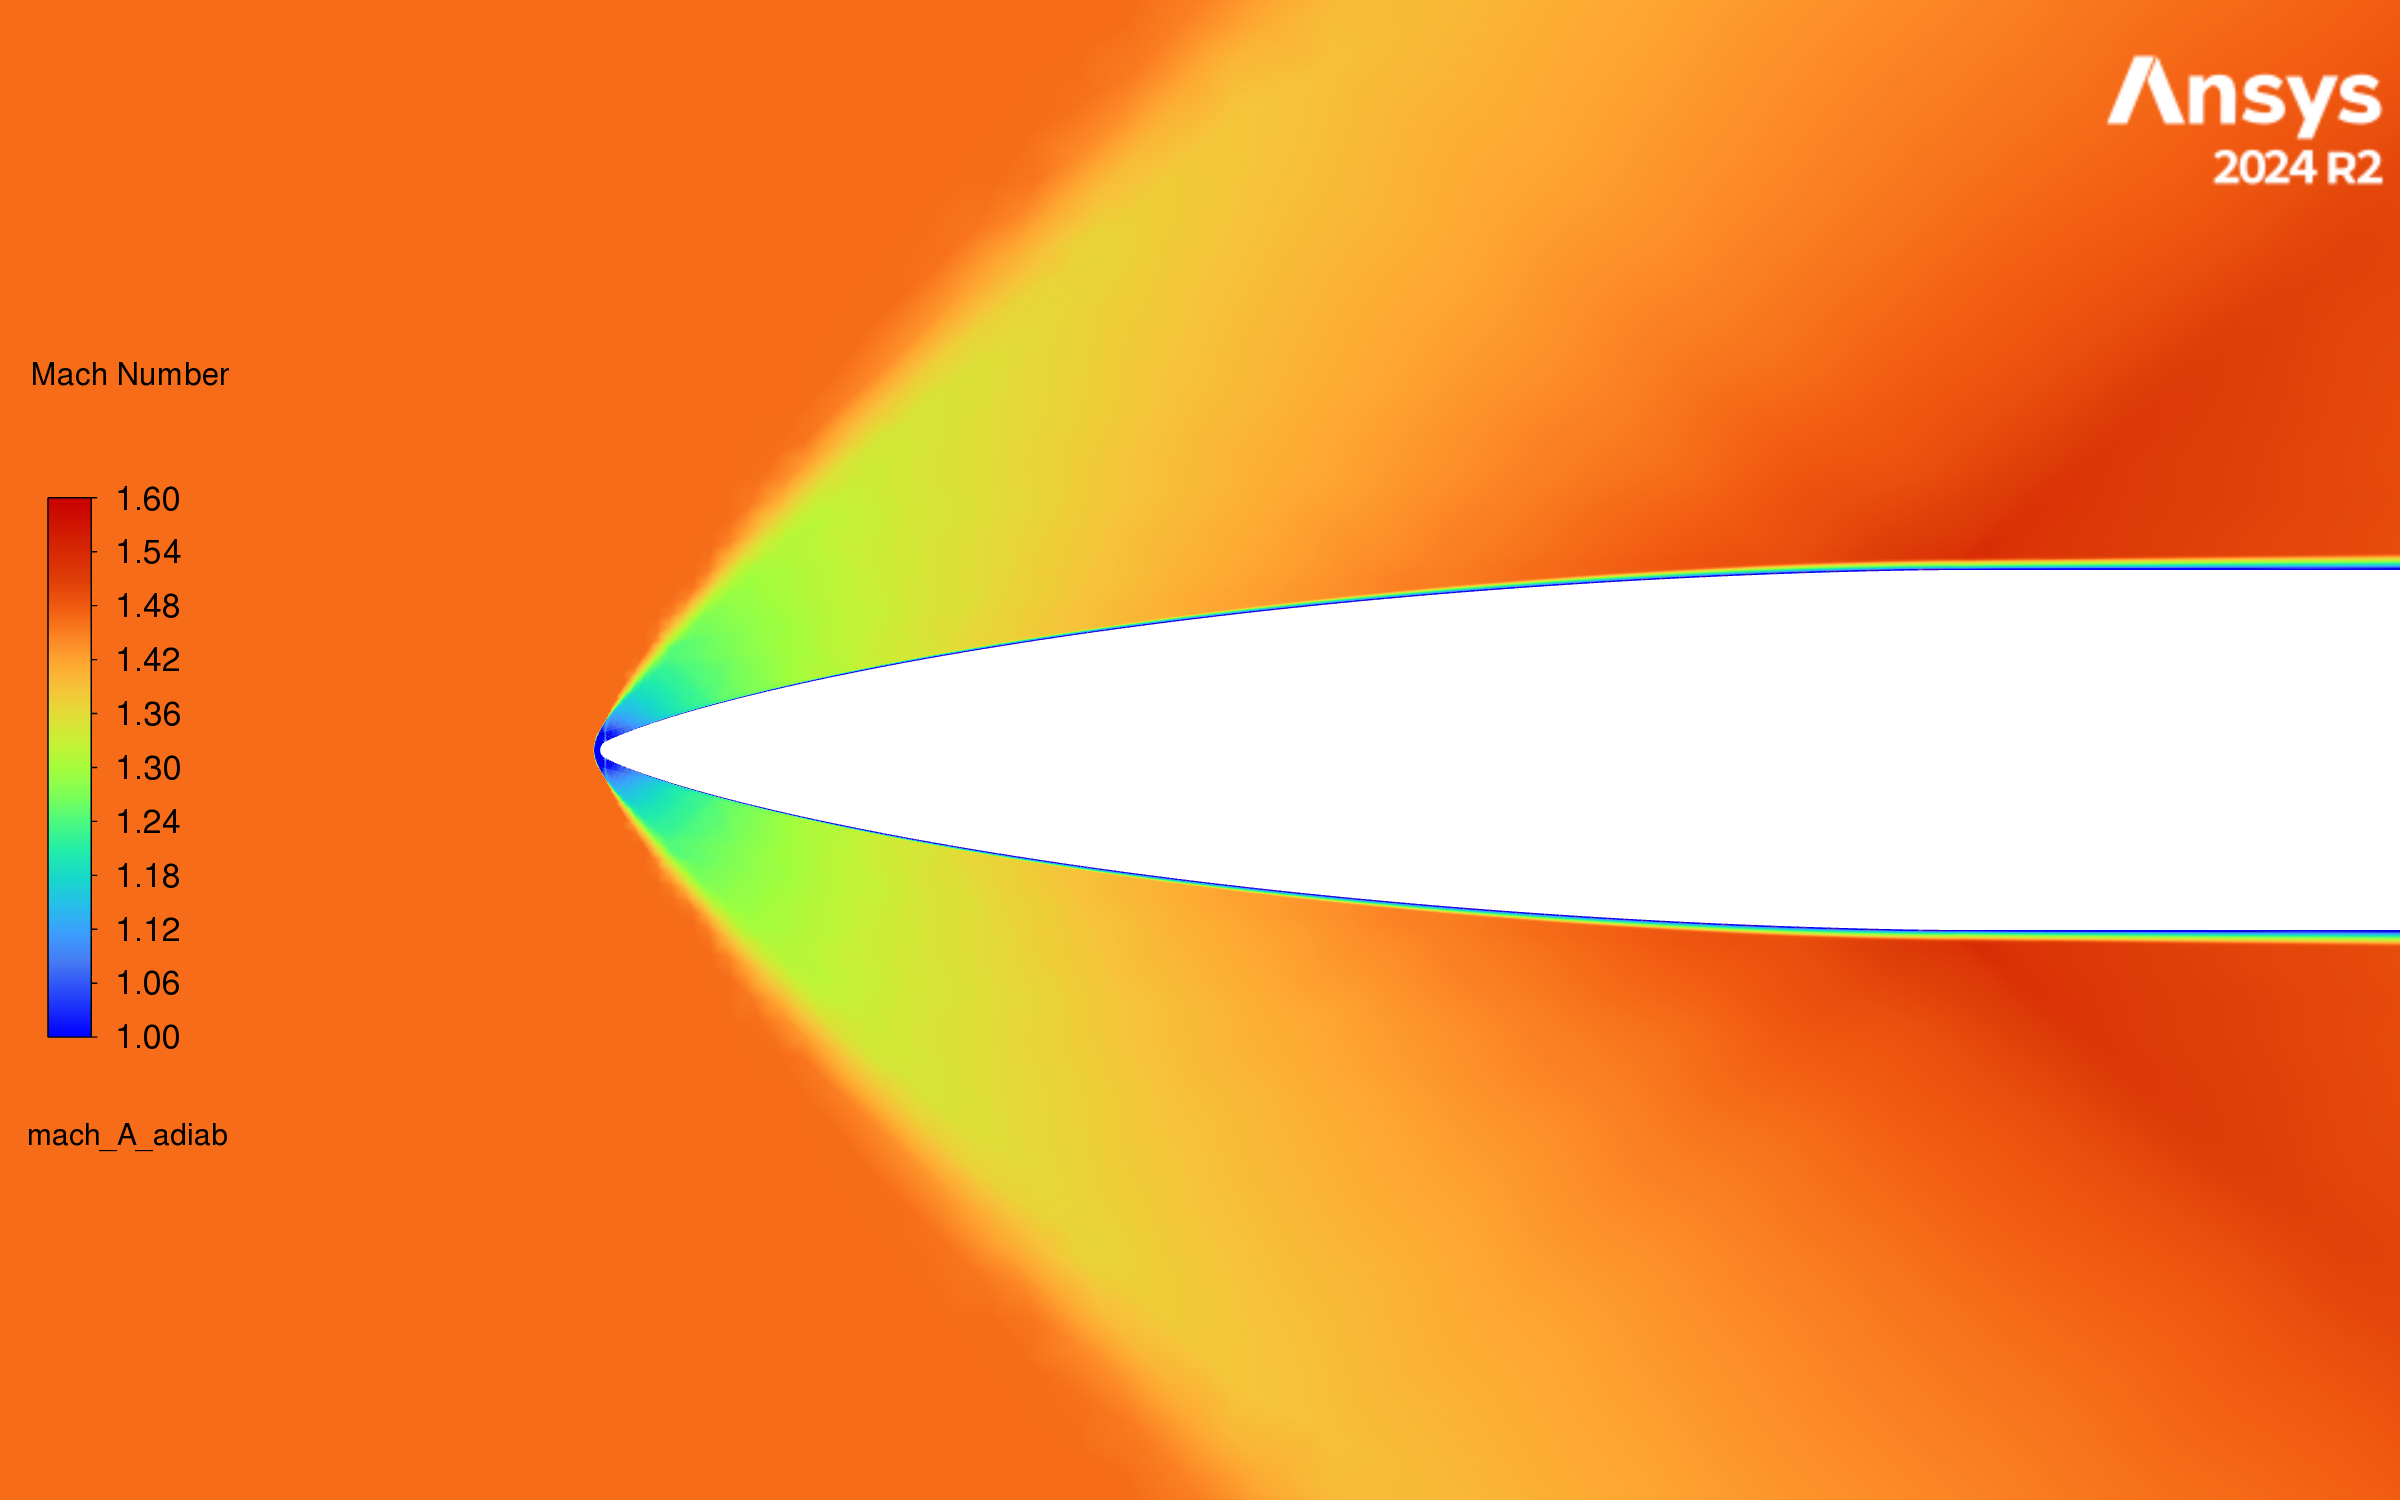
\includegraphics[width=\linewidth]{fluent_mach_A_adiab}
\caption{Design A.}
\end{subfigure}\hfill
\begin{subfigure}[t]{0.49\linewidth}
\centering
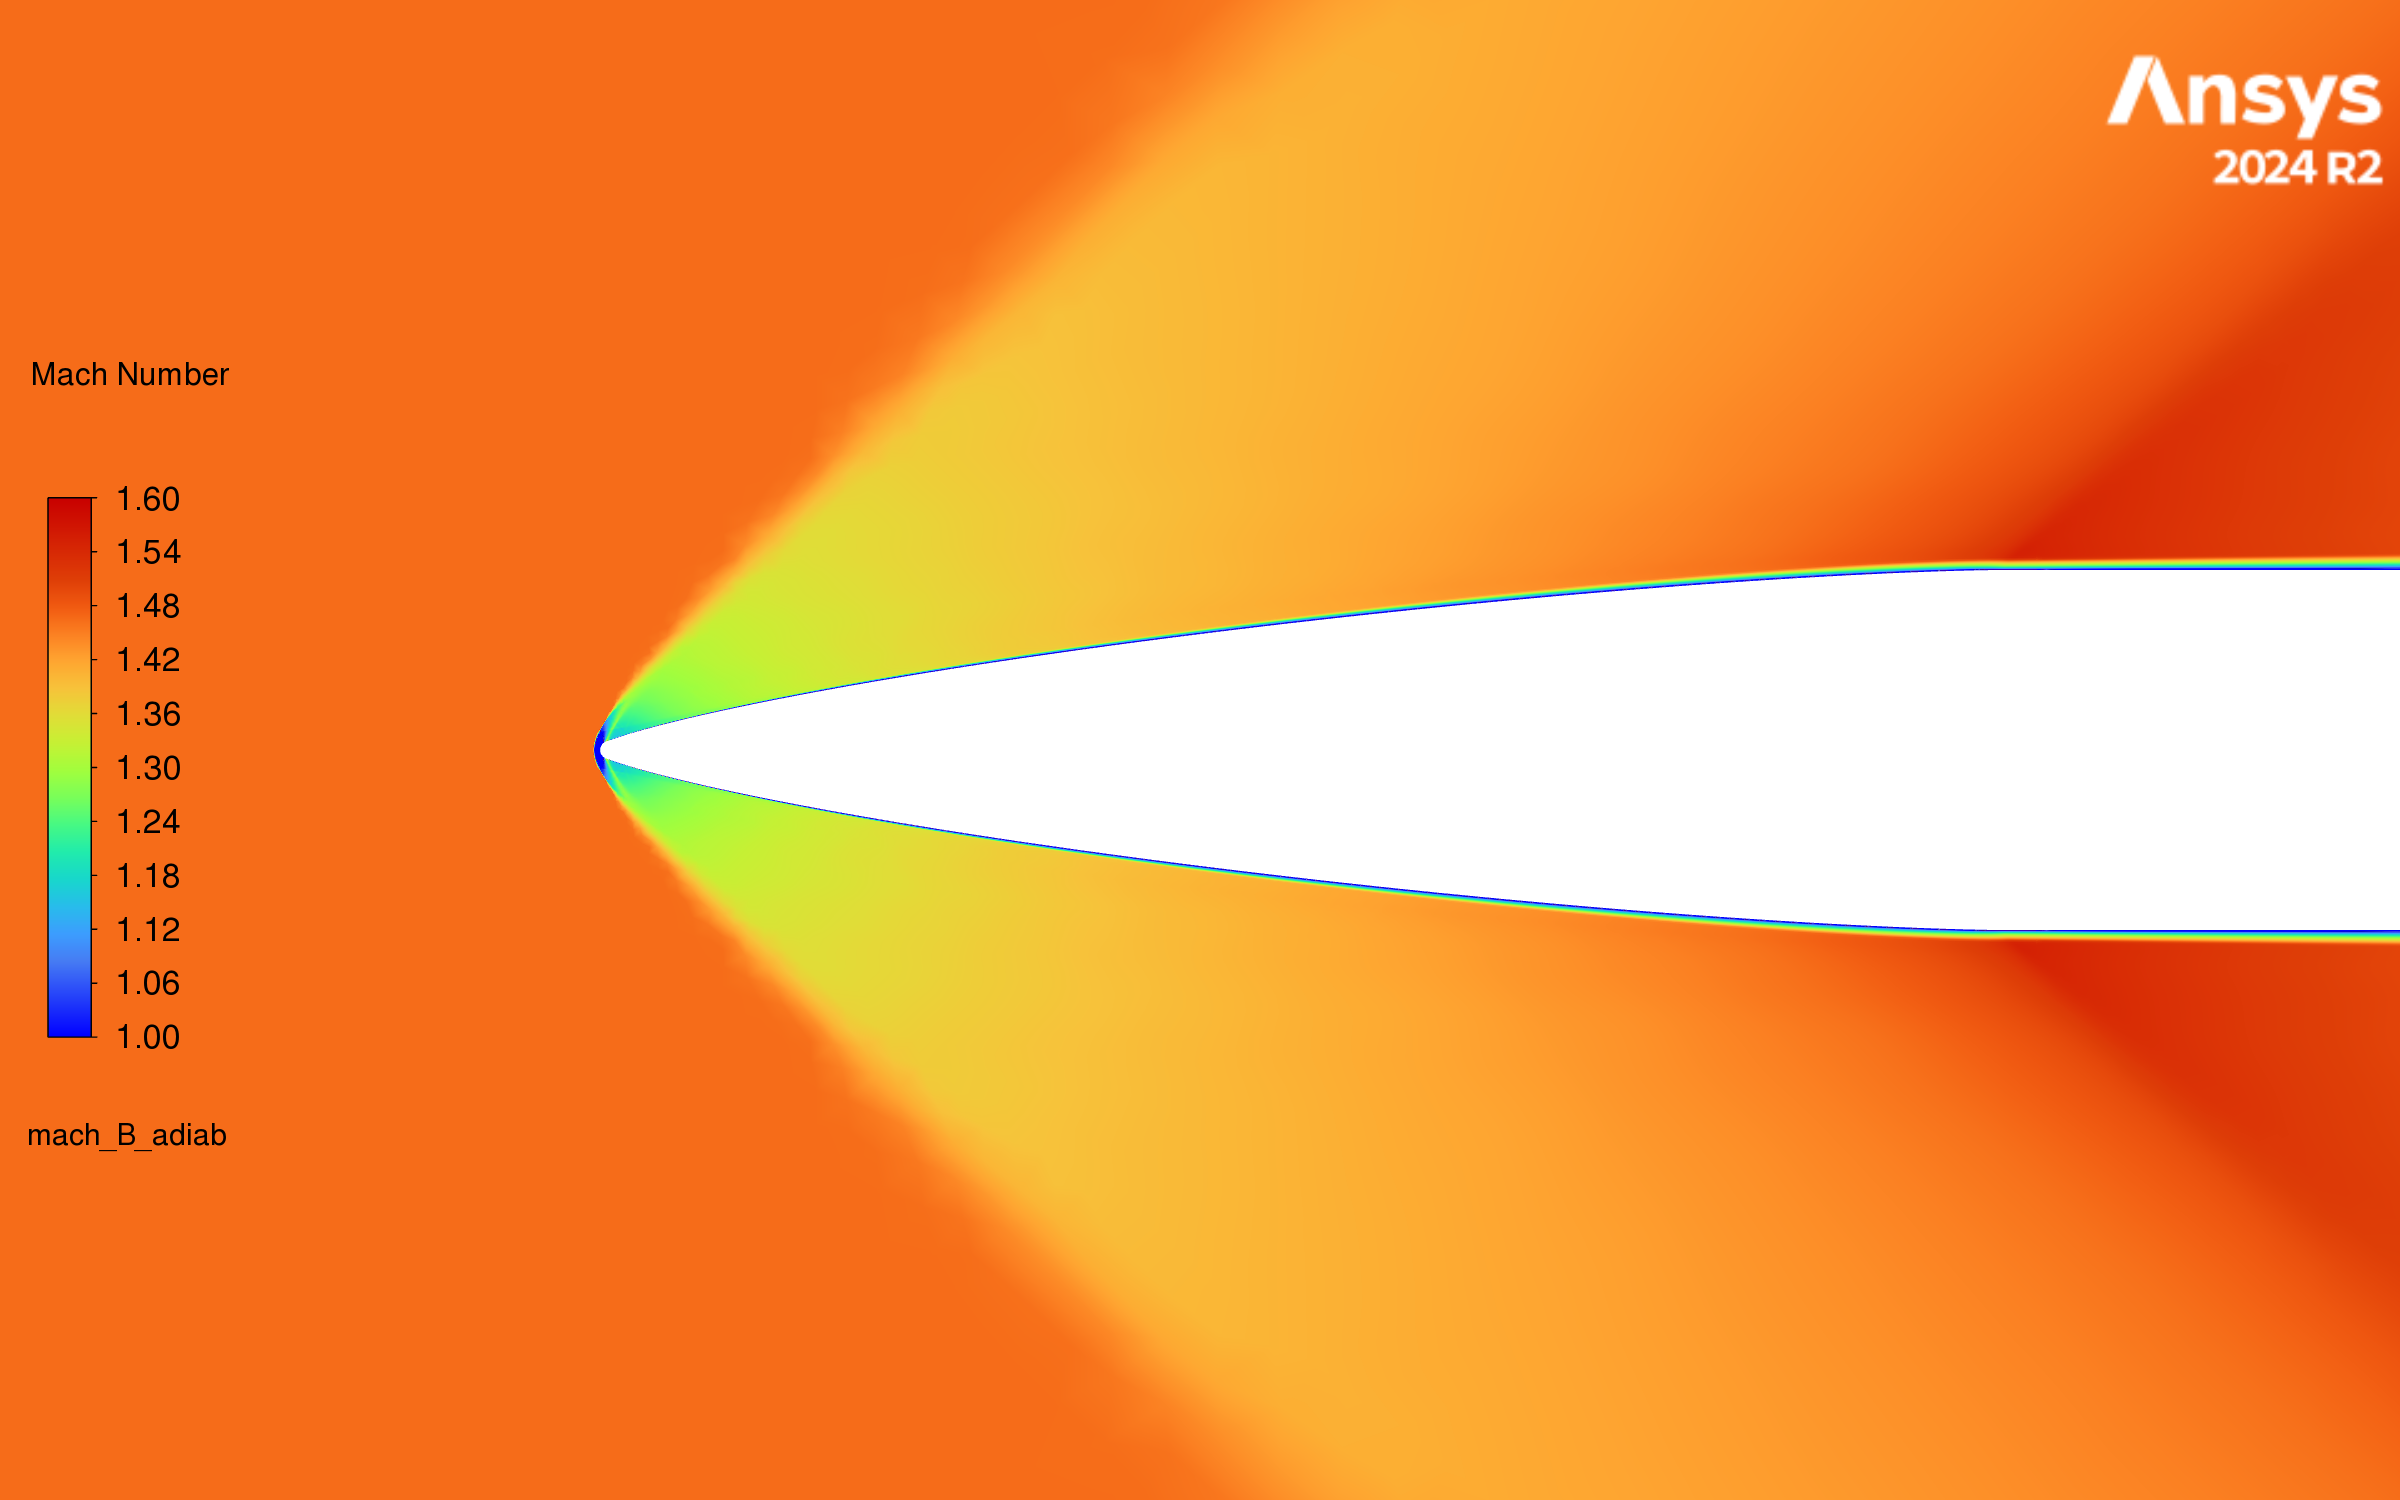
\includegraphics[width=\linewidth]{fluent_mach_B_adiab}
\caption{Design B.}
\end{subfigure}
\caption{Mach number around the nose at burnout (Fluent). Yellow and green: the air slowed down by the bow
shock and the front of the nose.}
\label{fig:mach}
\end{figure}

\begin{figure}[H]
\centering
\begin{subfigure}[t]{0.49\linewidth}
\centering
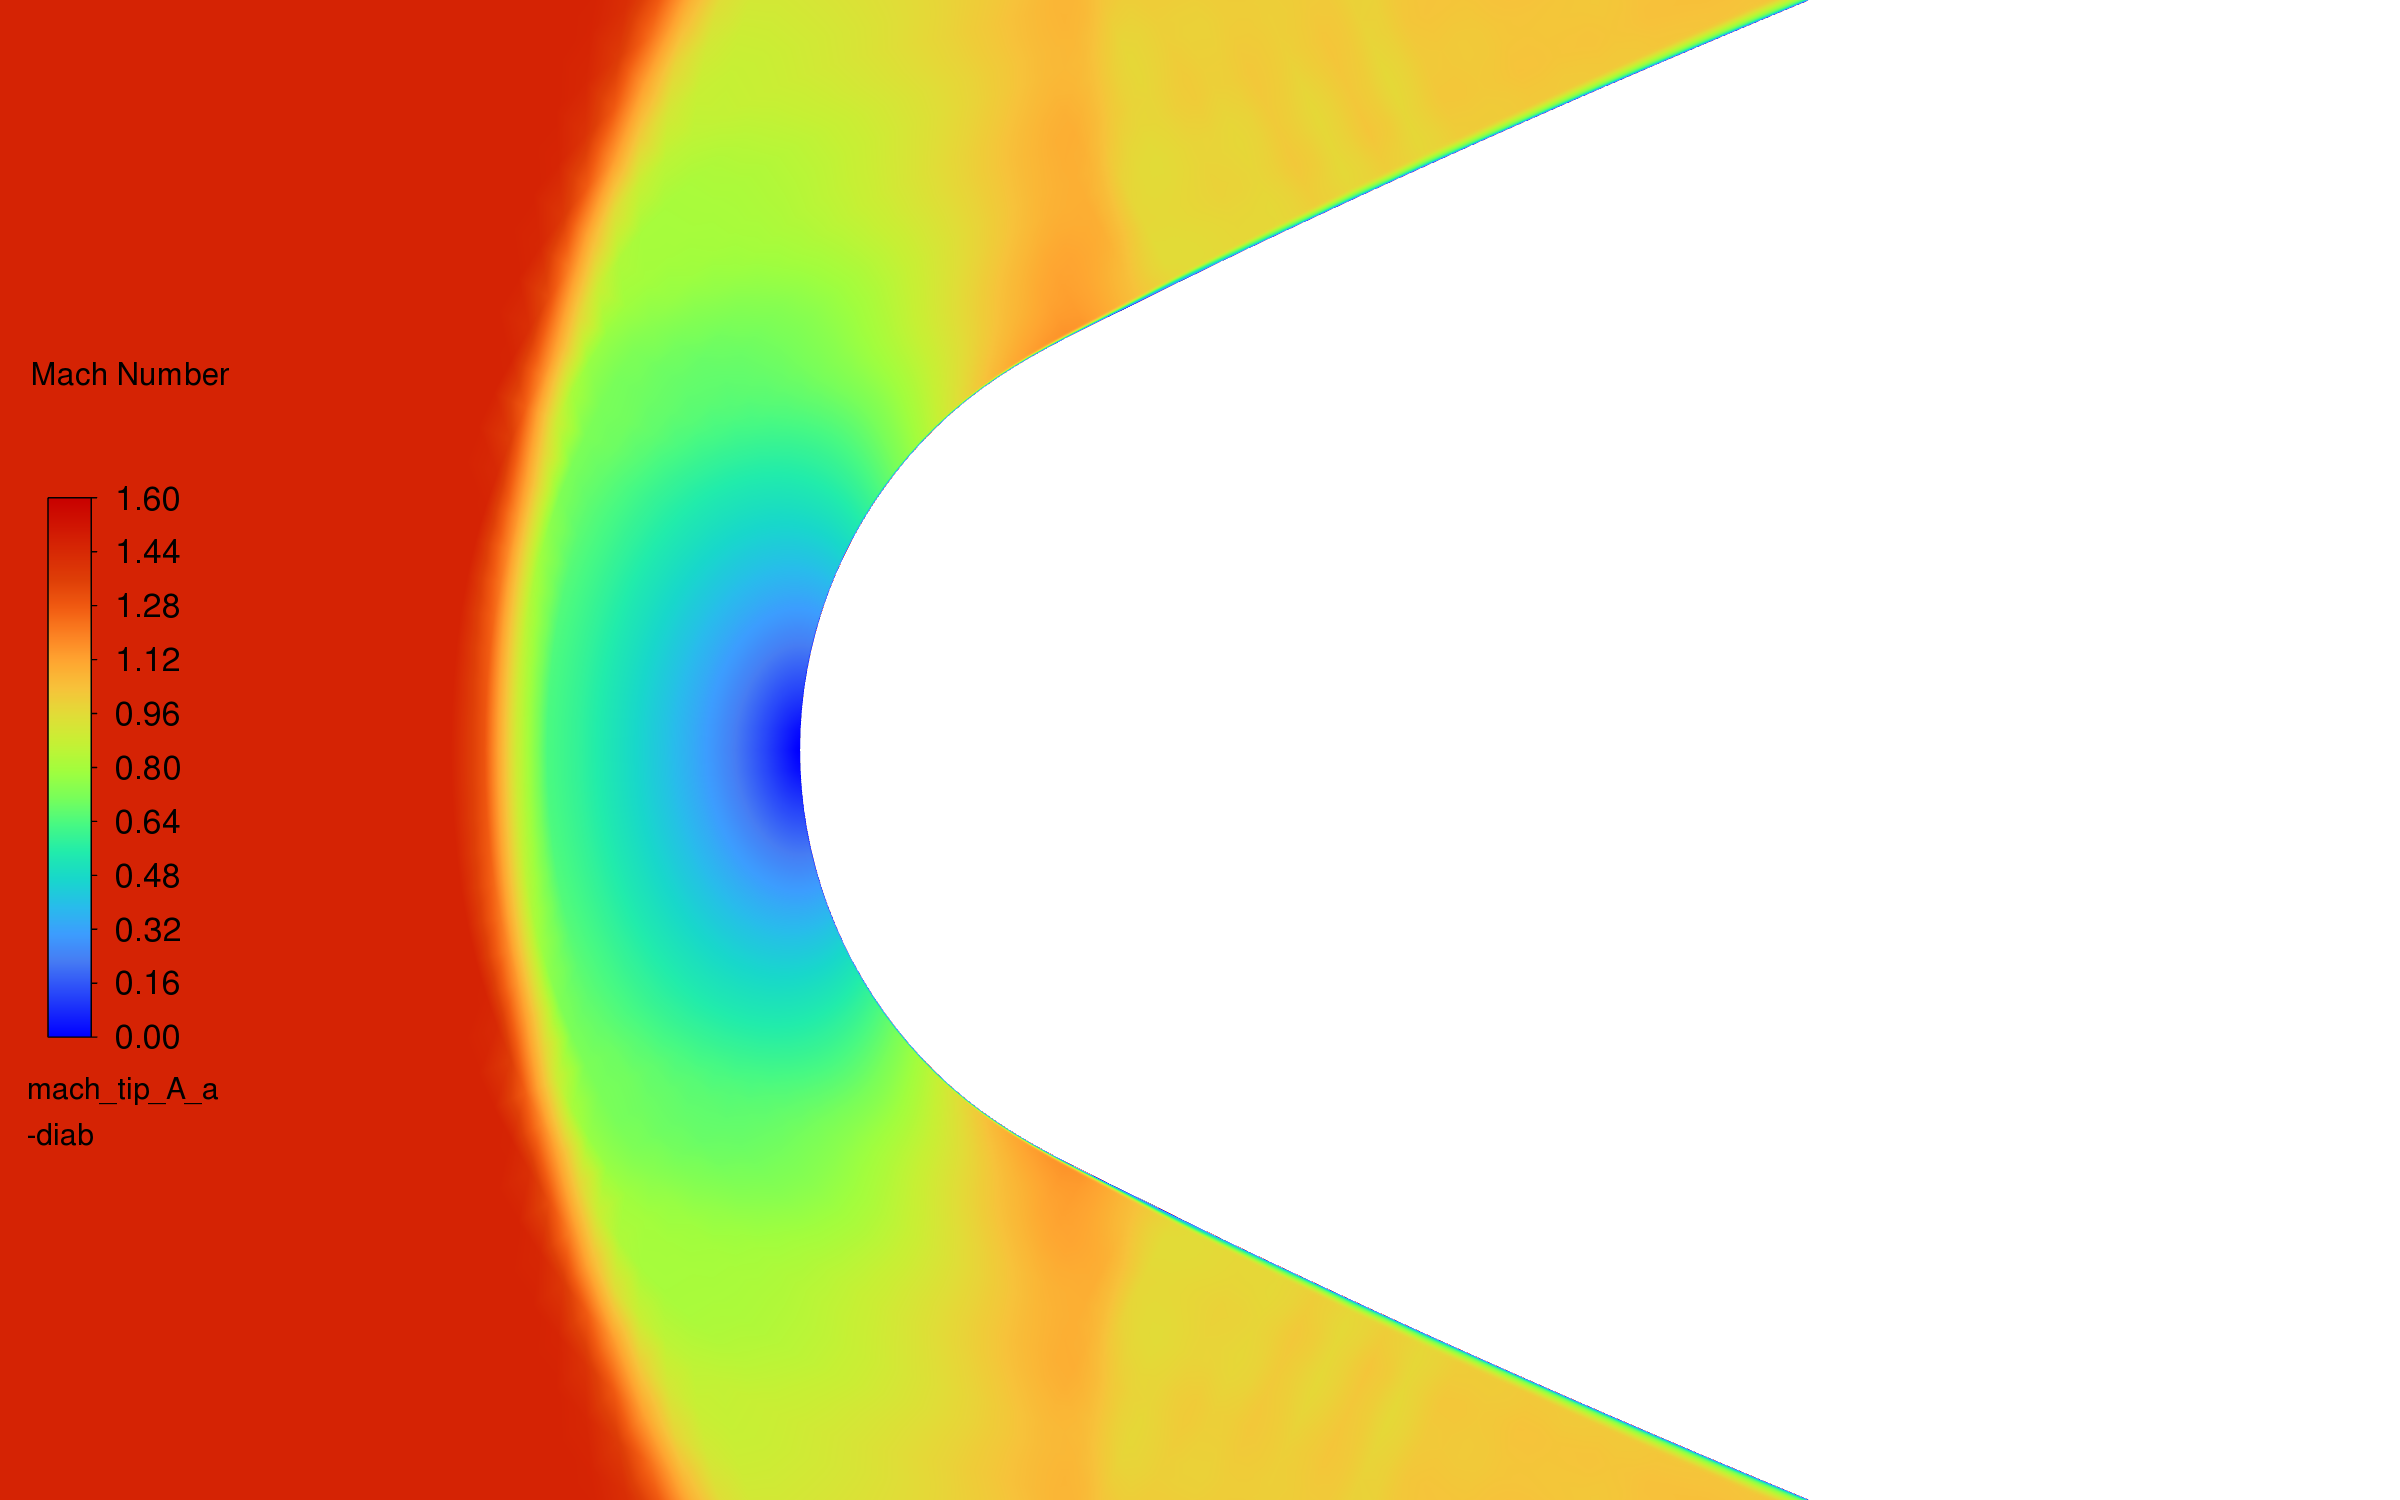
\includegraphics[width=\linewidth]{fluent_mach_tip_A_adiab}
\caption{Design A.}
\end{subfigure}\hfill
\begin{subfigure}[t]{0.49\linewidth}
\centering
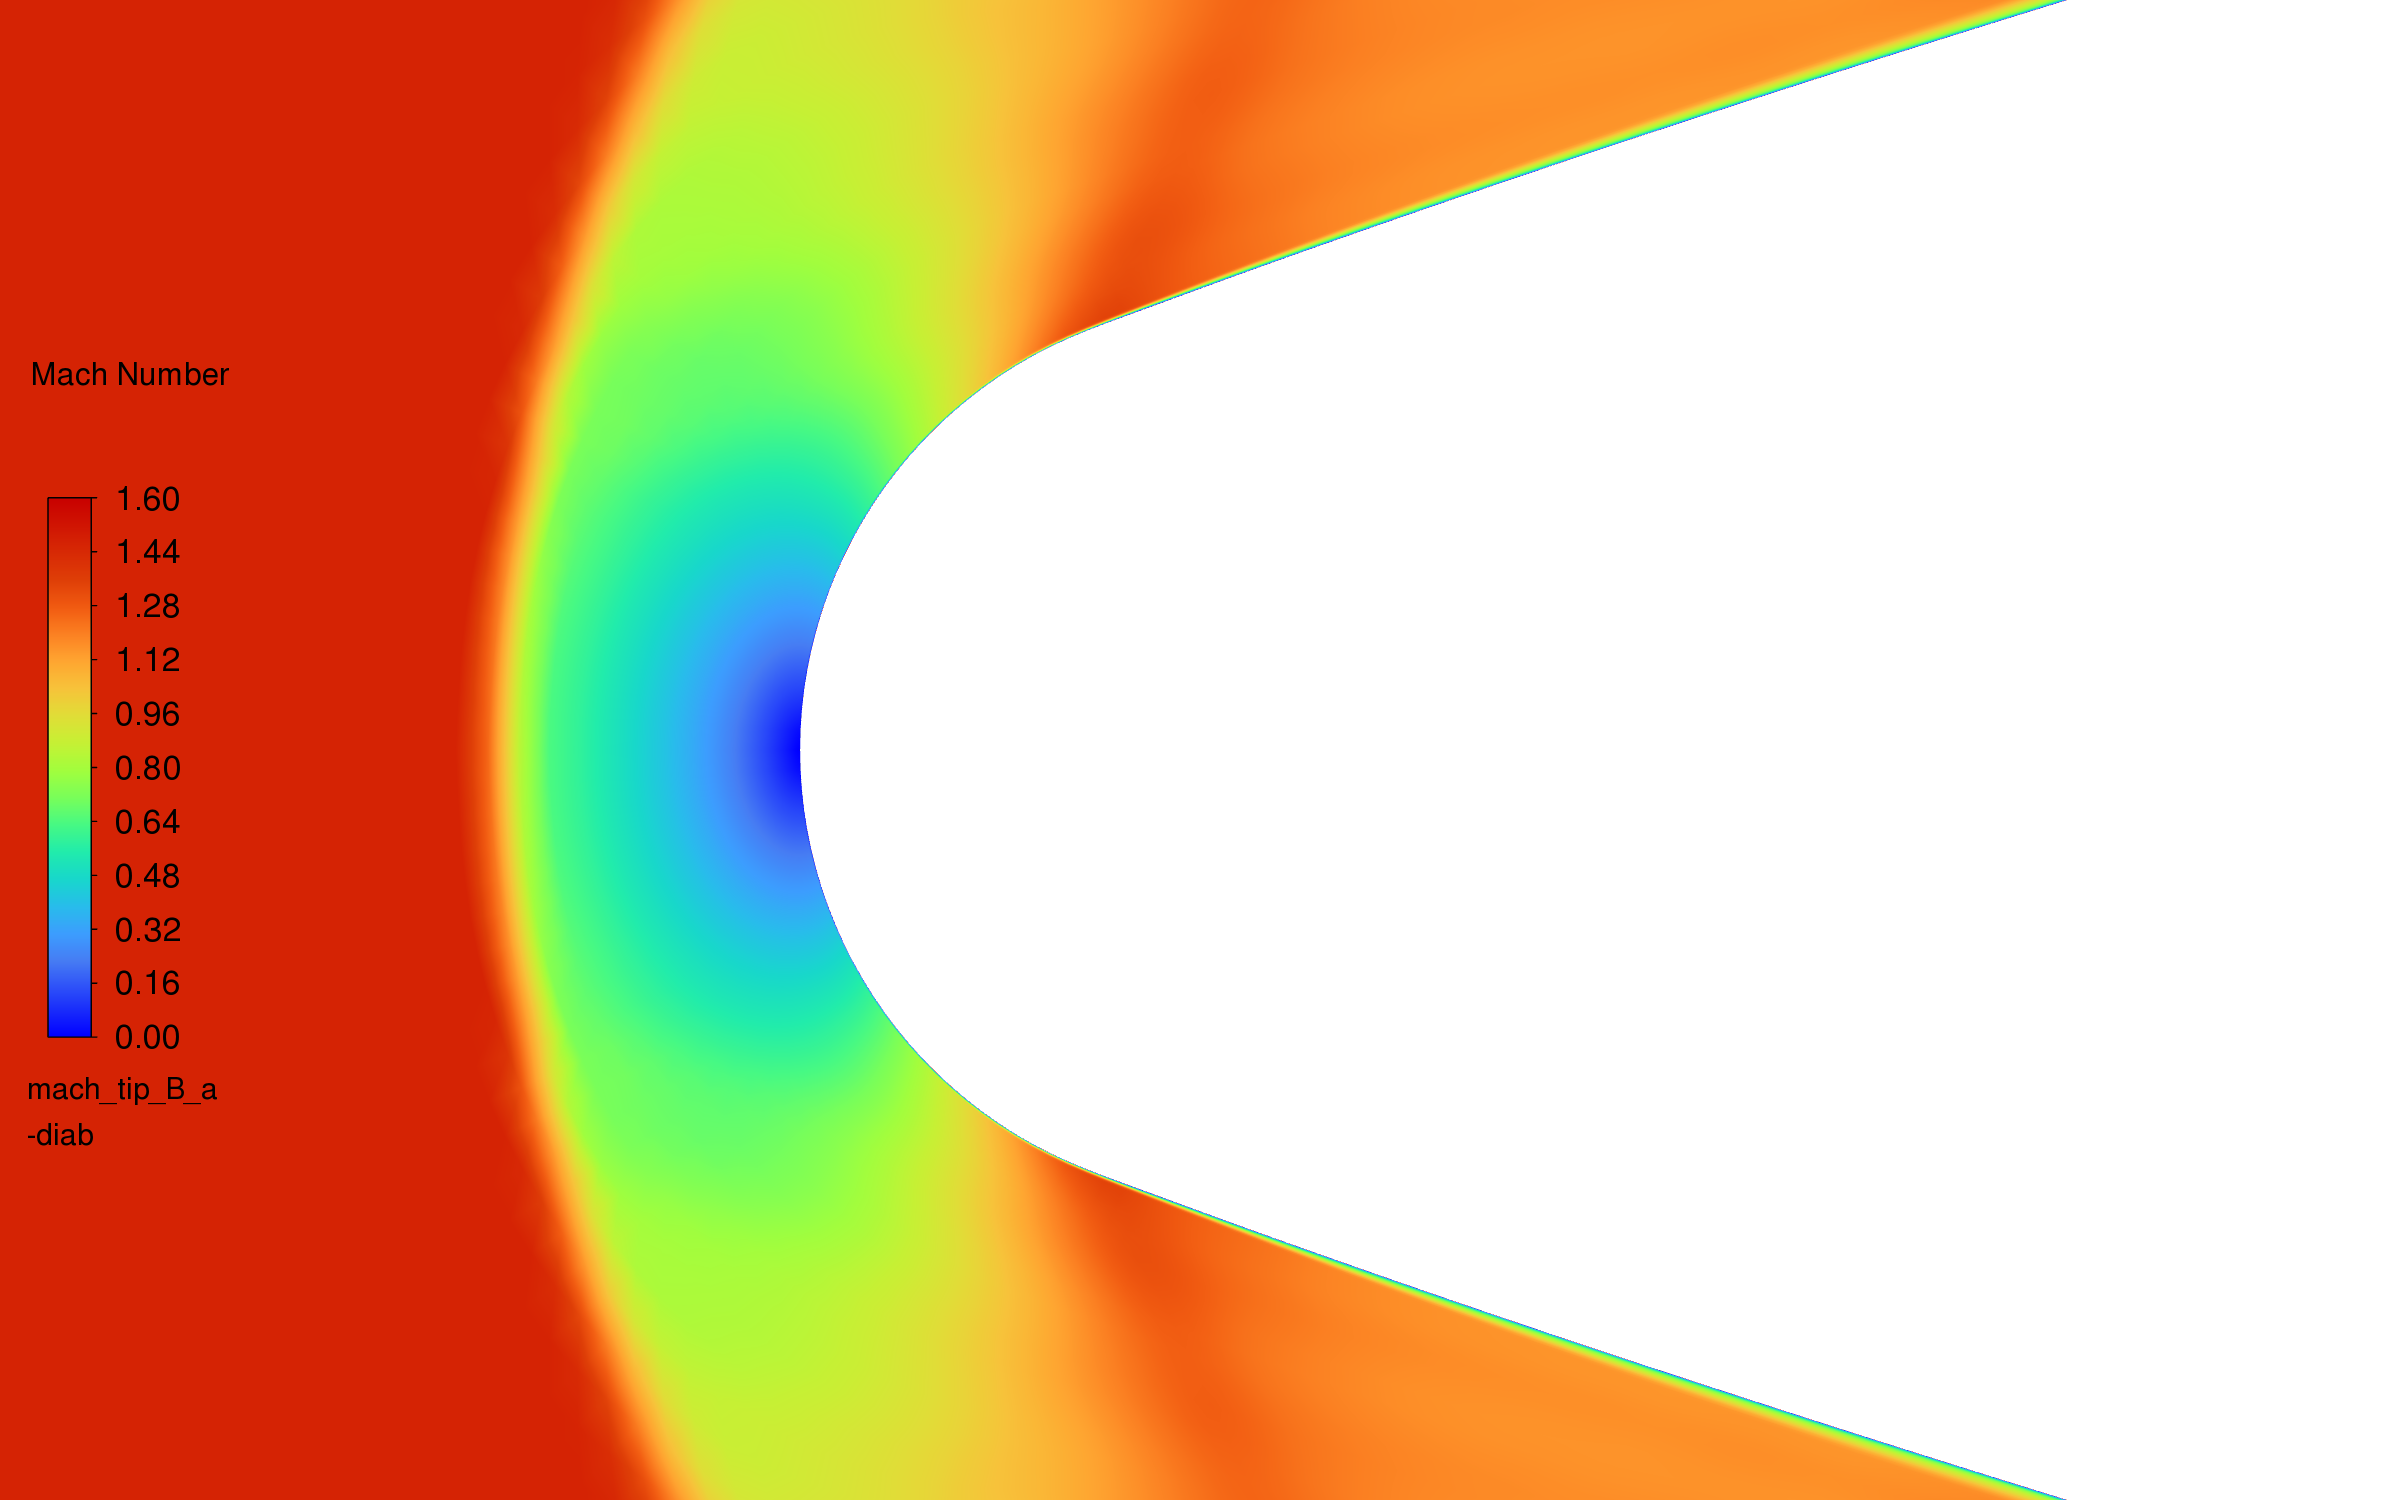
\includegraphics[width=\linewidth]{fluent_mach_tip_B_adiab}
\caption{Design B.}
\end{subfigure}
\caption{Mach number around the tip at burnout (Fluent). The bow shock stands just ahead of the rounded
tip, with a small subsonic region behind it.}
\label{fig:machtip}
\end{figure}

\begin{figure}[H]
\centering
\begin{subfigure}[t]{0.49\linewidth}
\centering
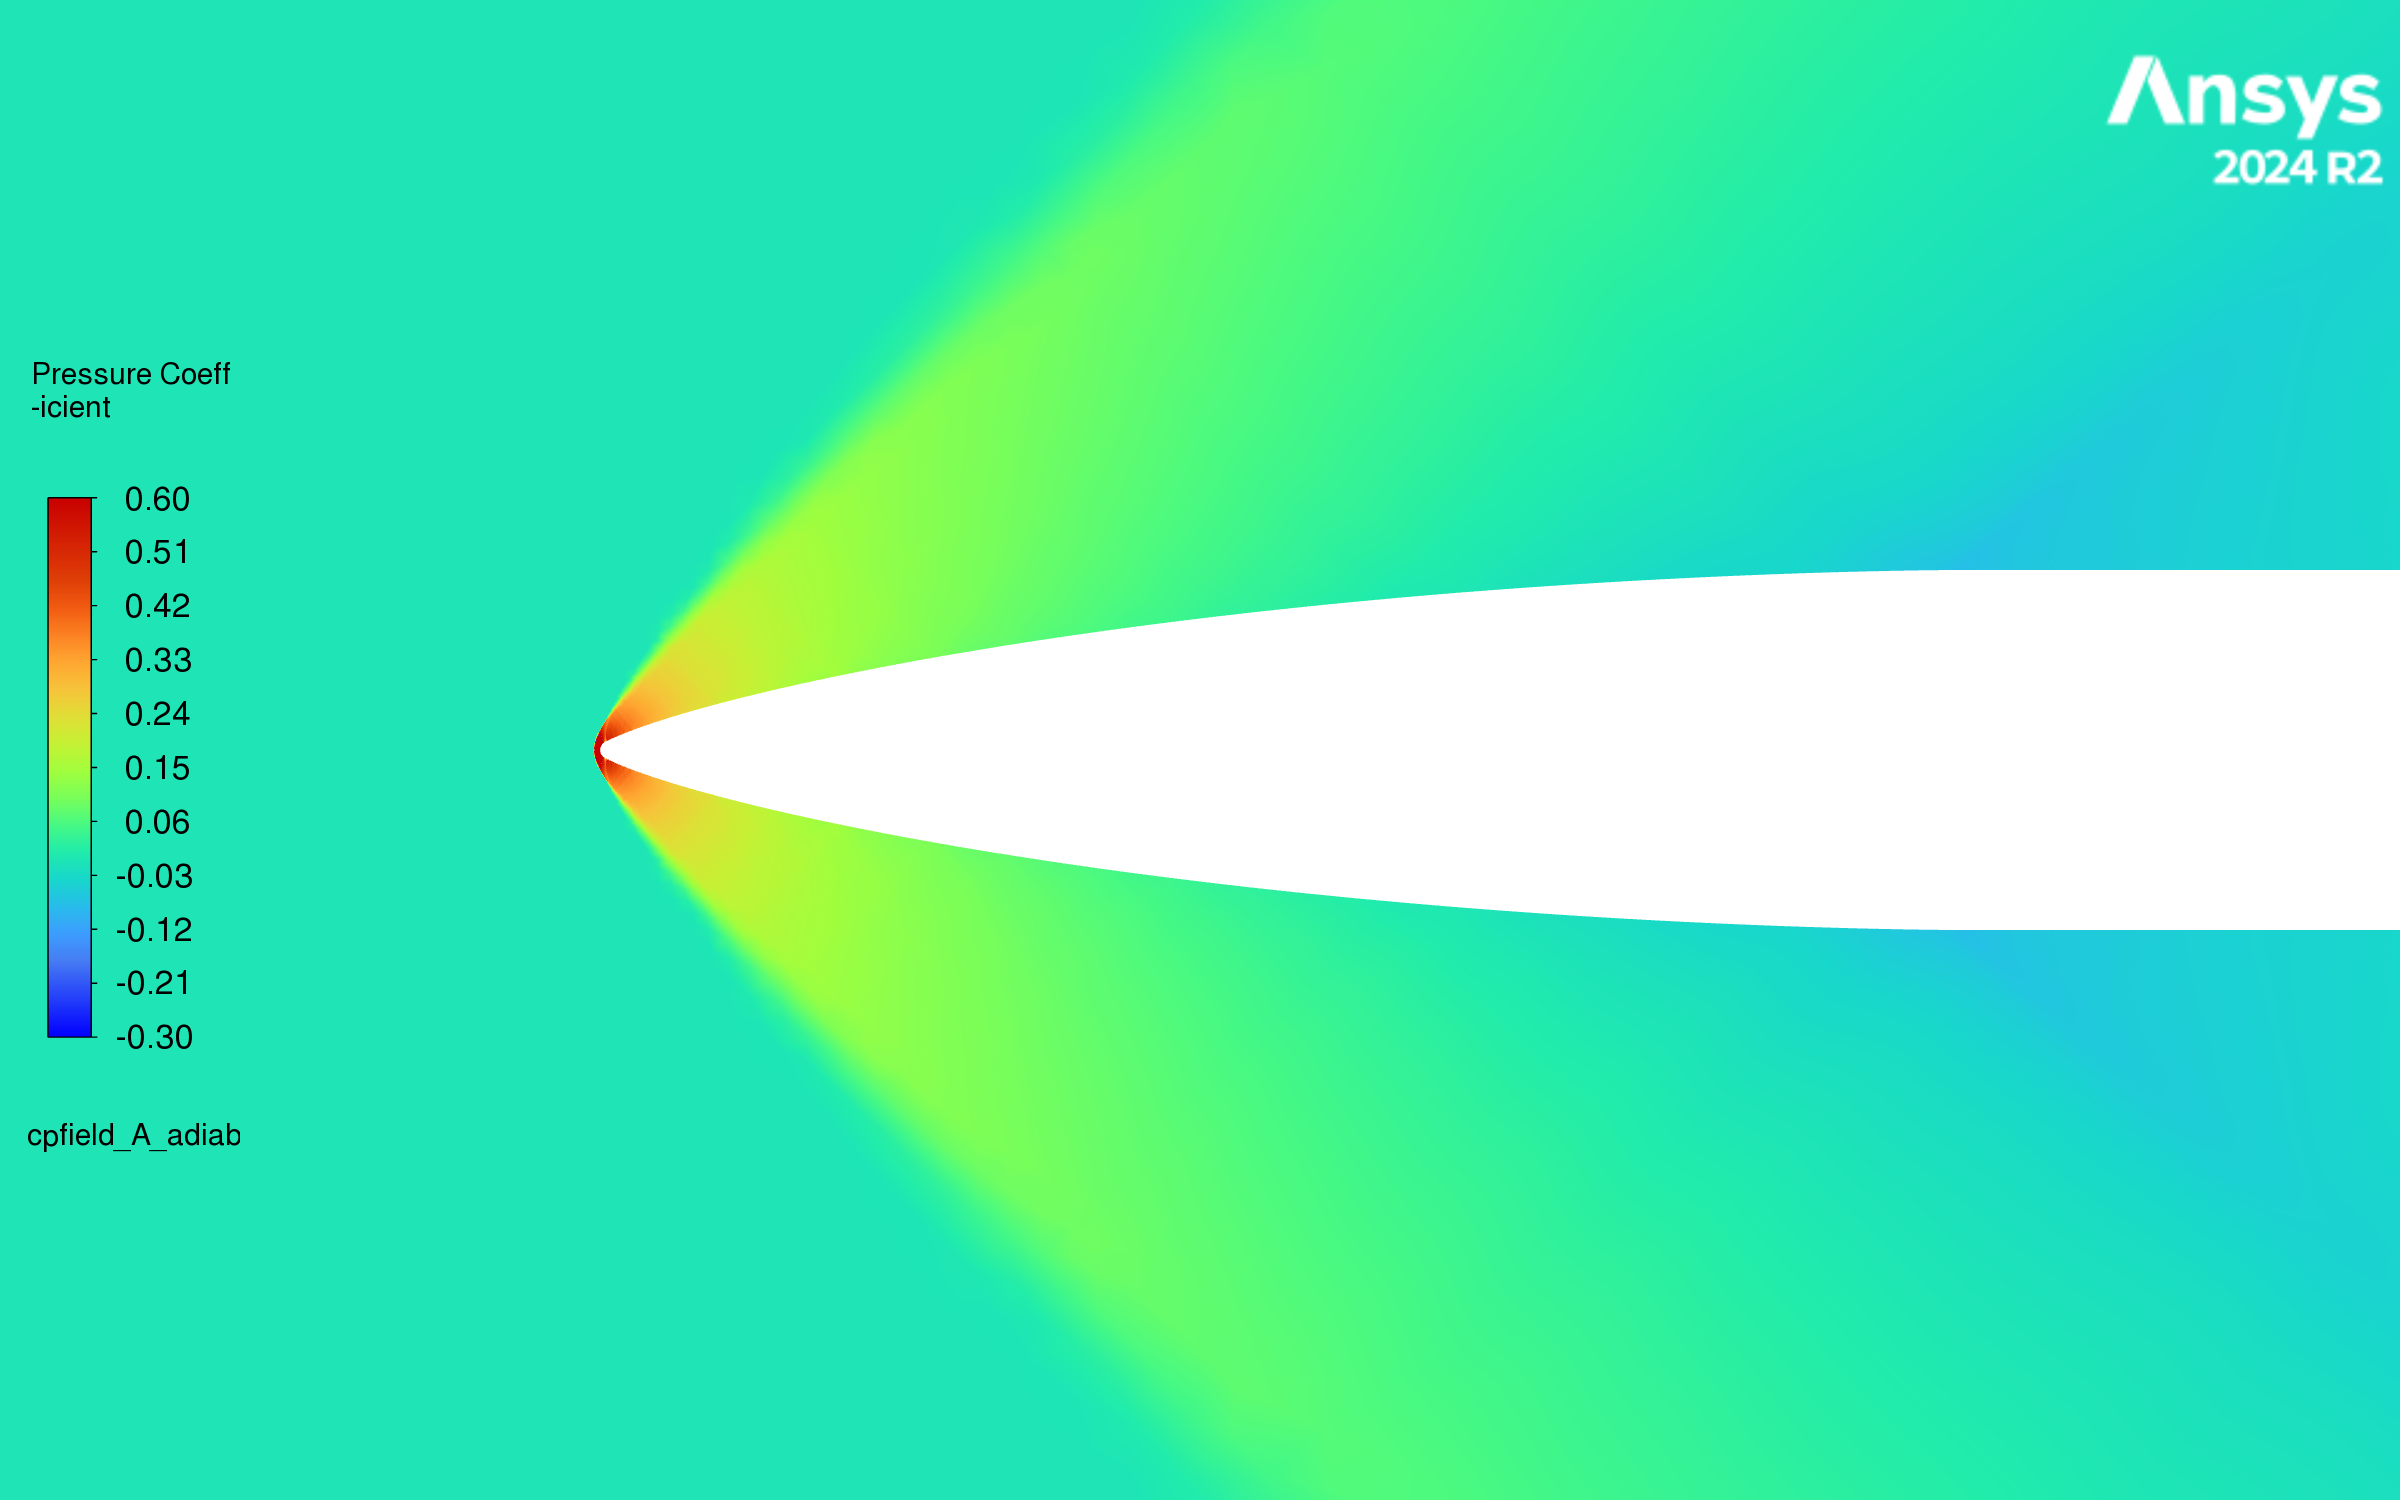
\includegraphics[width=\linewidth]{fluent_cpfield_A_adiab}
\caption{Design A.}
\end{subfigure}\hfill
\begin{subfigure}[t]{0.49\linewidth}
\centering
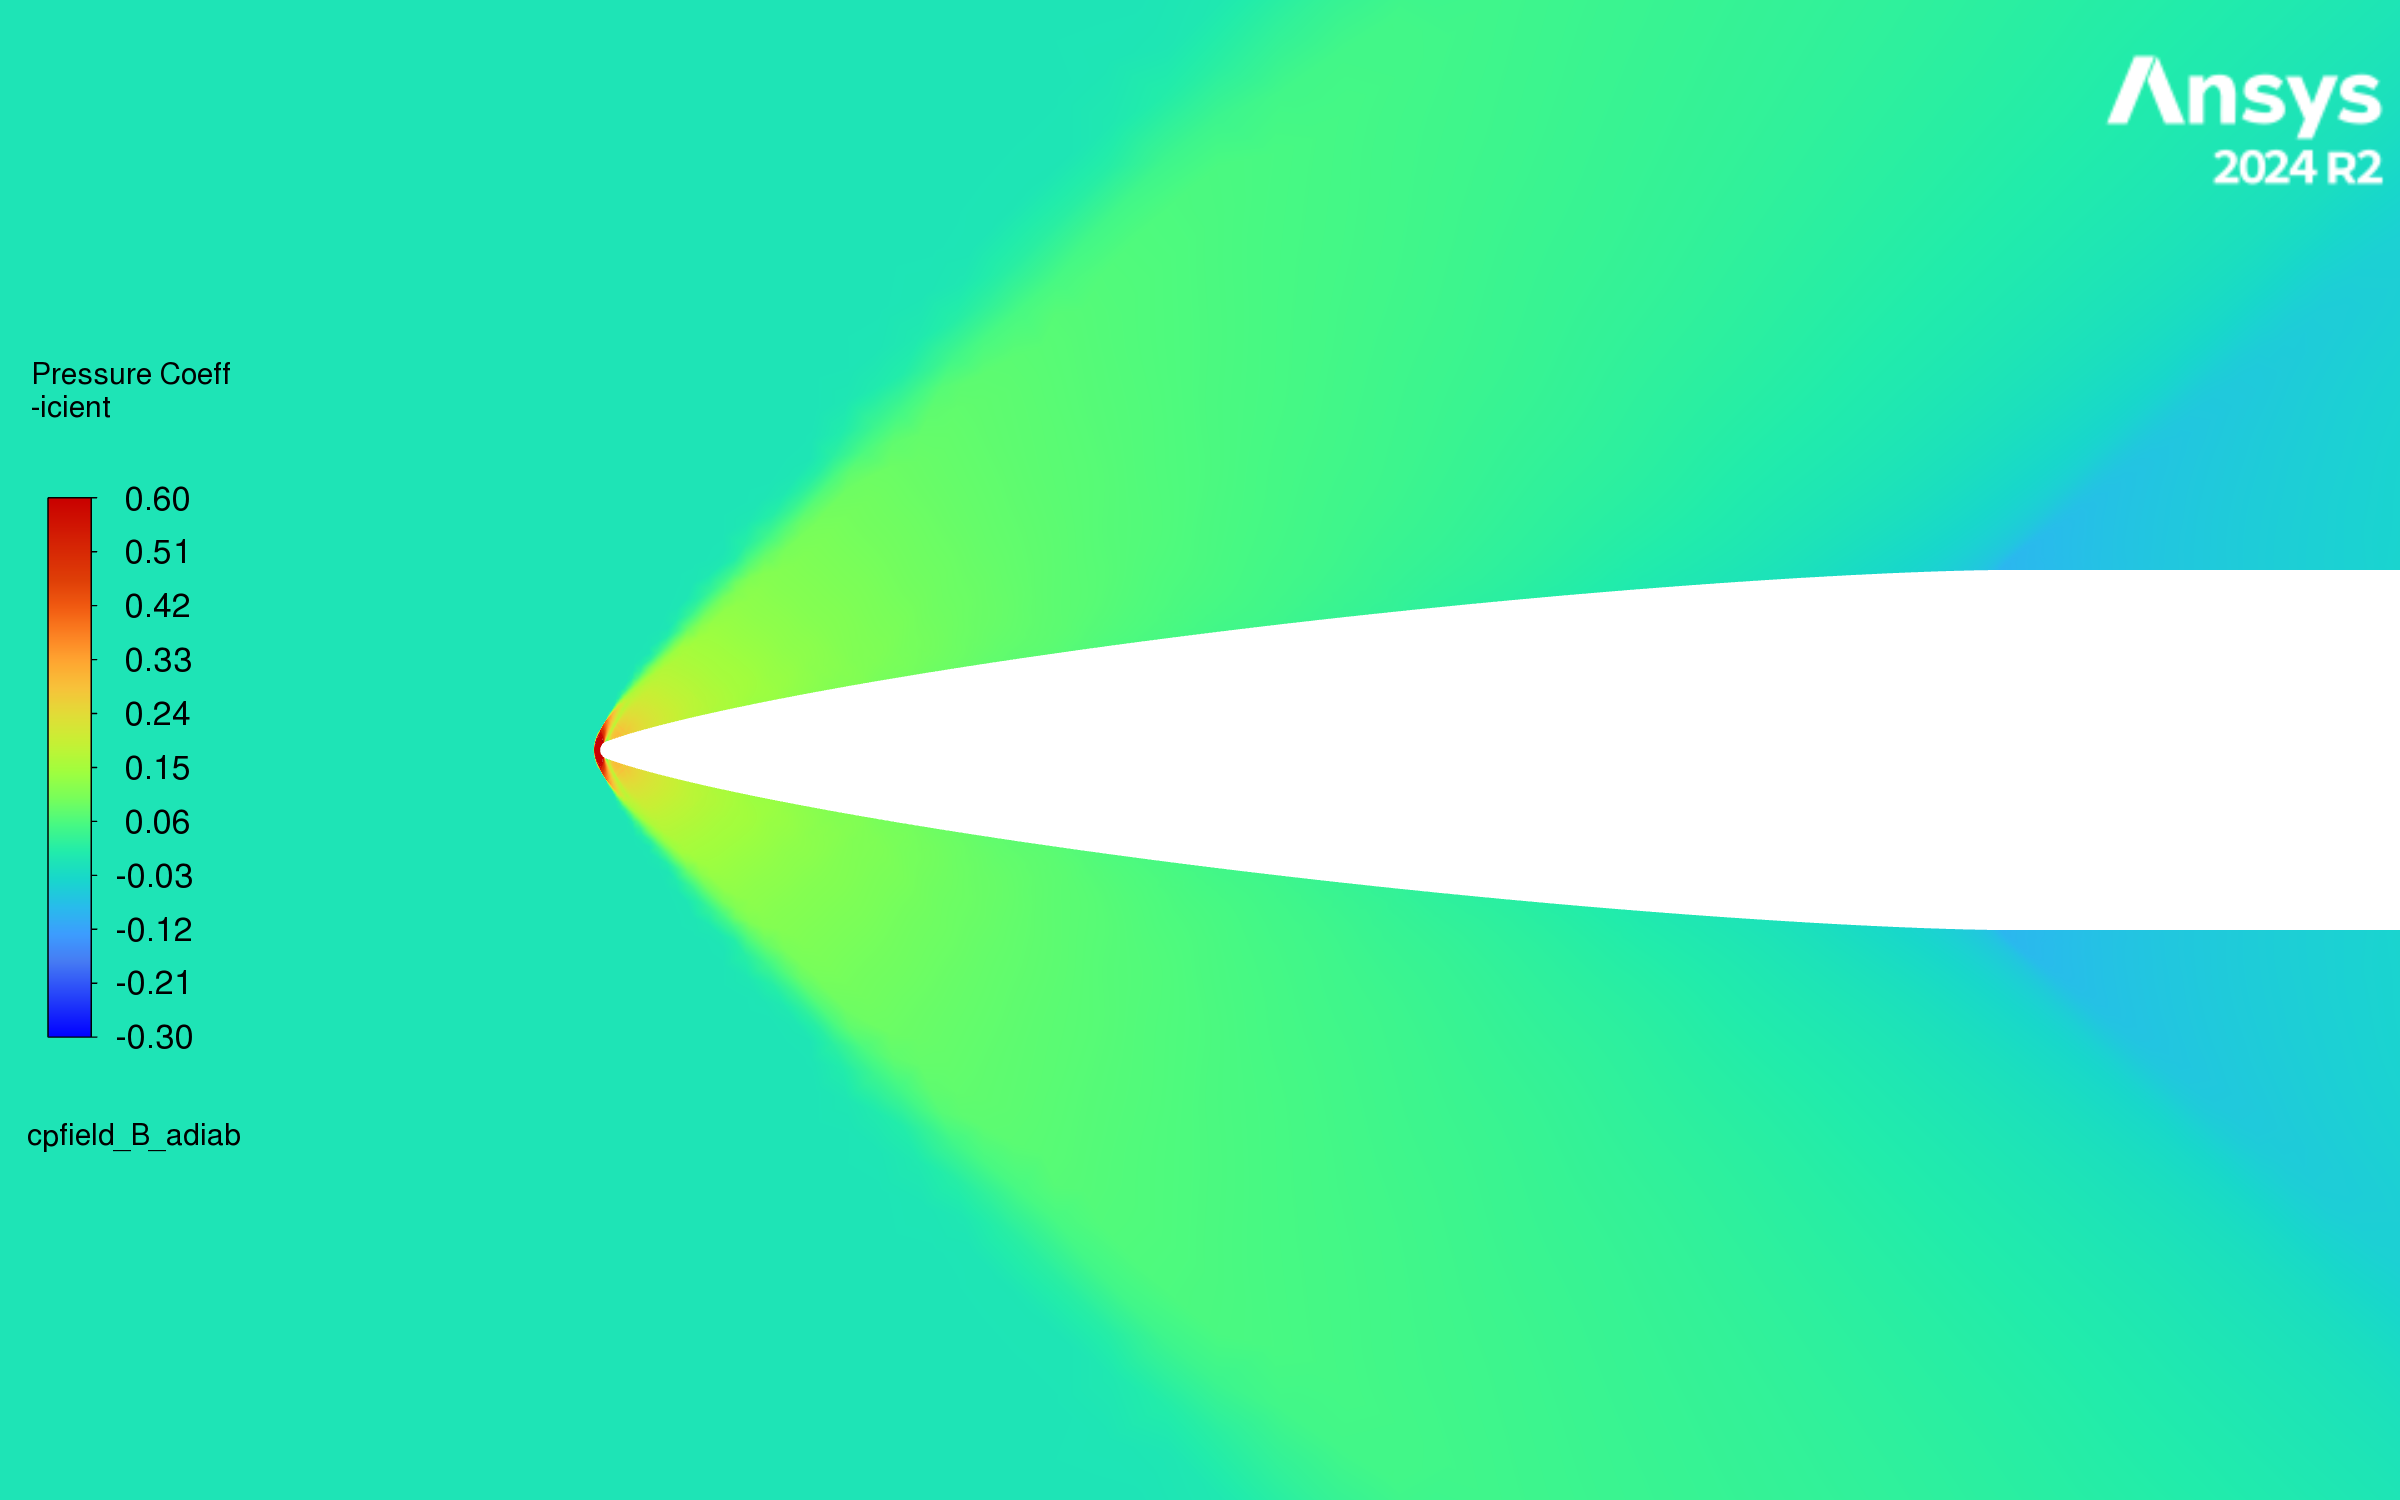
\includegraphics[width=\linewidth]{fluent_cpfield_B_adiab}
\caption{Design B.}
\end{subfigure}
\caption{Pressure coefficient around the nose at burnout (Fluent), $C_p = (p - p_\infty)/q$. Warm colours:
pressure above the outside pressure, which pushes the nose back.}
\label{fig:cpfield}
\end{figure}

\begin{figure}[H]
\centering
\begin{subfigure}[t]{\linewidth}
\centering
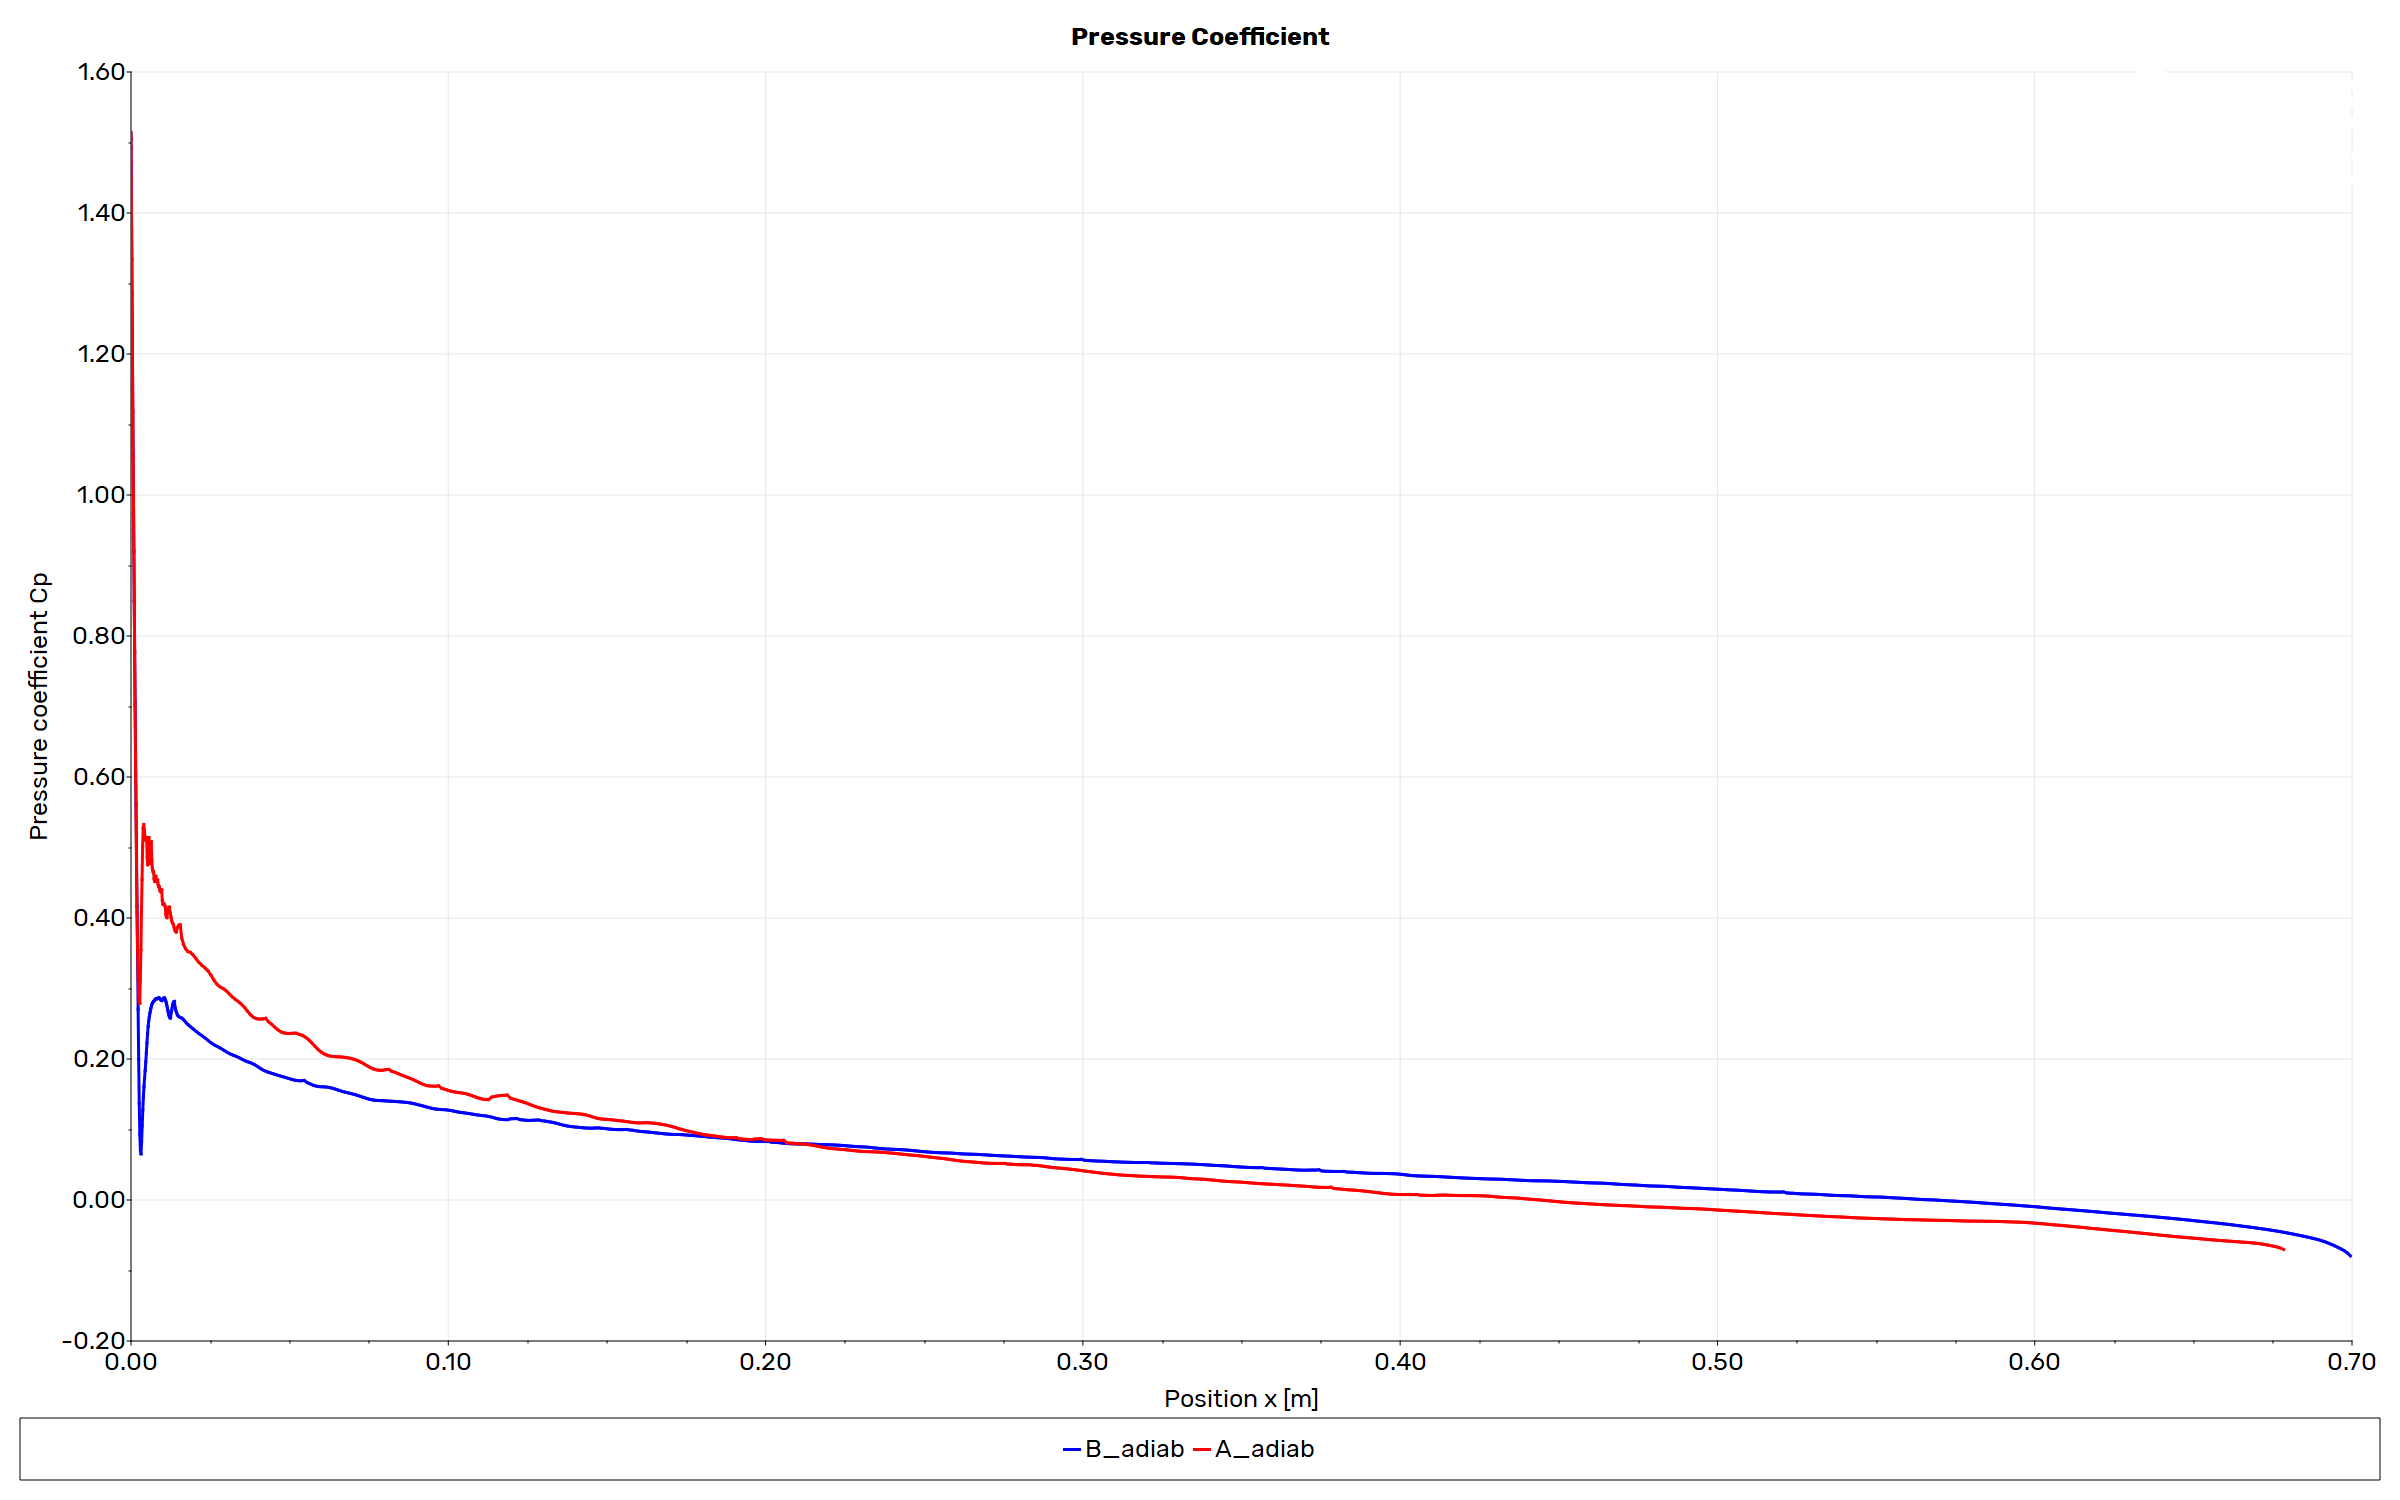
\includegraphics[width=\linewidth]{fluent_cp_AB_adiab}
\caption{Burnout, $M = \val{pt-M147-M}$.}
\end{subfigure}

\medskip
\begin{subfigure}[t]{\linewidth}
\centering
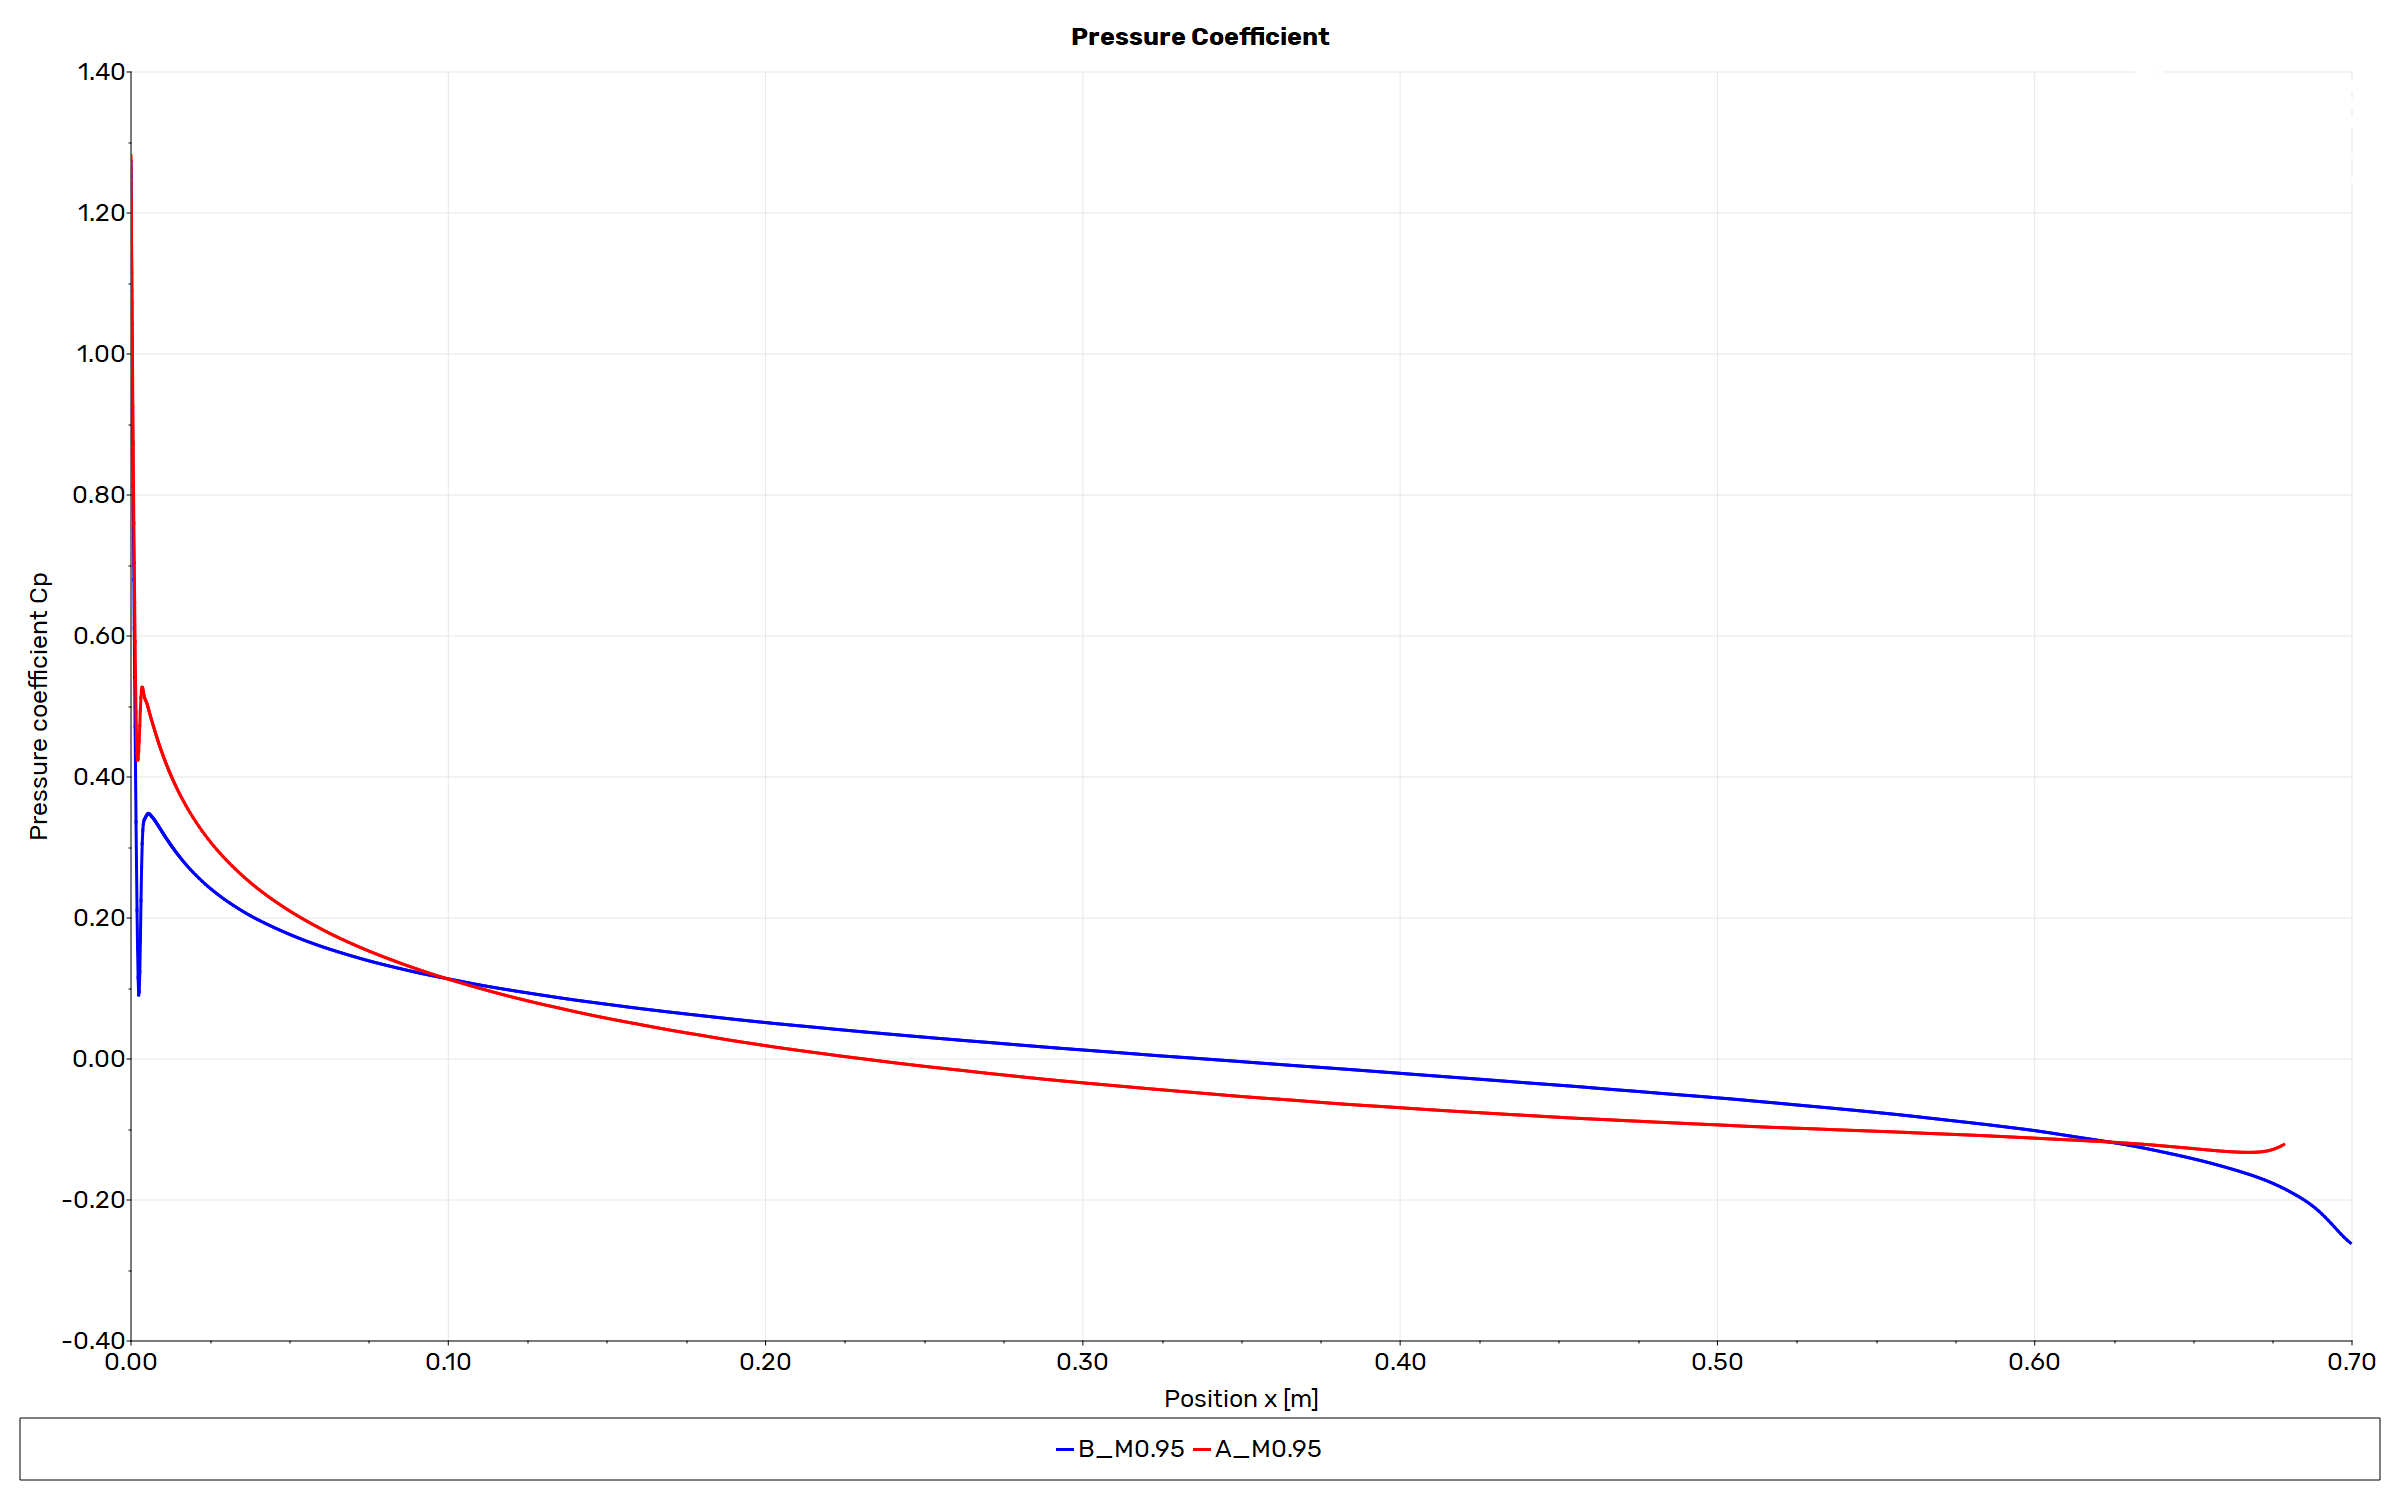
\includegraphics[width=\linewidth]{fluent_cp_AB_M0.95}
\caption{Transonic, $M = 0.95$.}
\end{subfigure}
\caption{Pressure coefficient along the wall, design A (red) and B (blue), Fluent. The $M = 1.20$ run lies
between the two.}
\label{fig:cp}
\end{figure}

\subsection{Below Mach 1: same drag}

At $M = 0.95$ no bow shock forms ahead of the nose (Figure~\ref{fig:mach095}). The pressure drag is only
about 5\,N for both designs (Table~\ref{tab:forces}), so the drag is almost all skin friction. The friction
along the wall is nearly the same for both noses (Figure~\ref{fig:cf}), so their drag is the same.

\begin{figure}[H]
\centering
\begin{subfigure}[t]{0.49\linewidth}
\centering
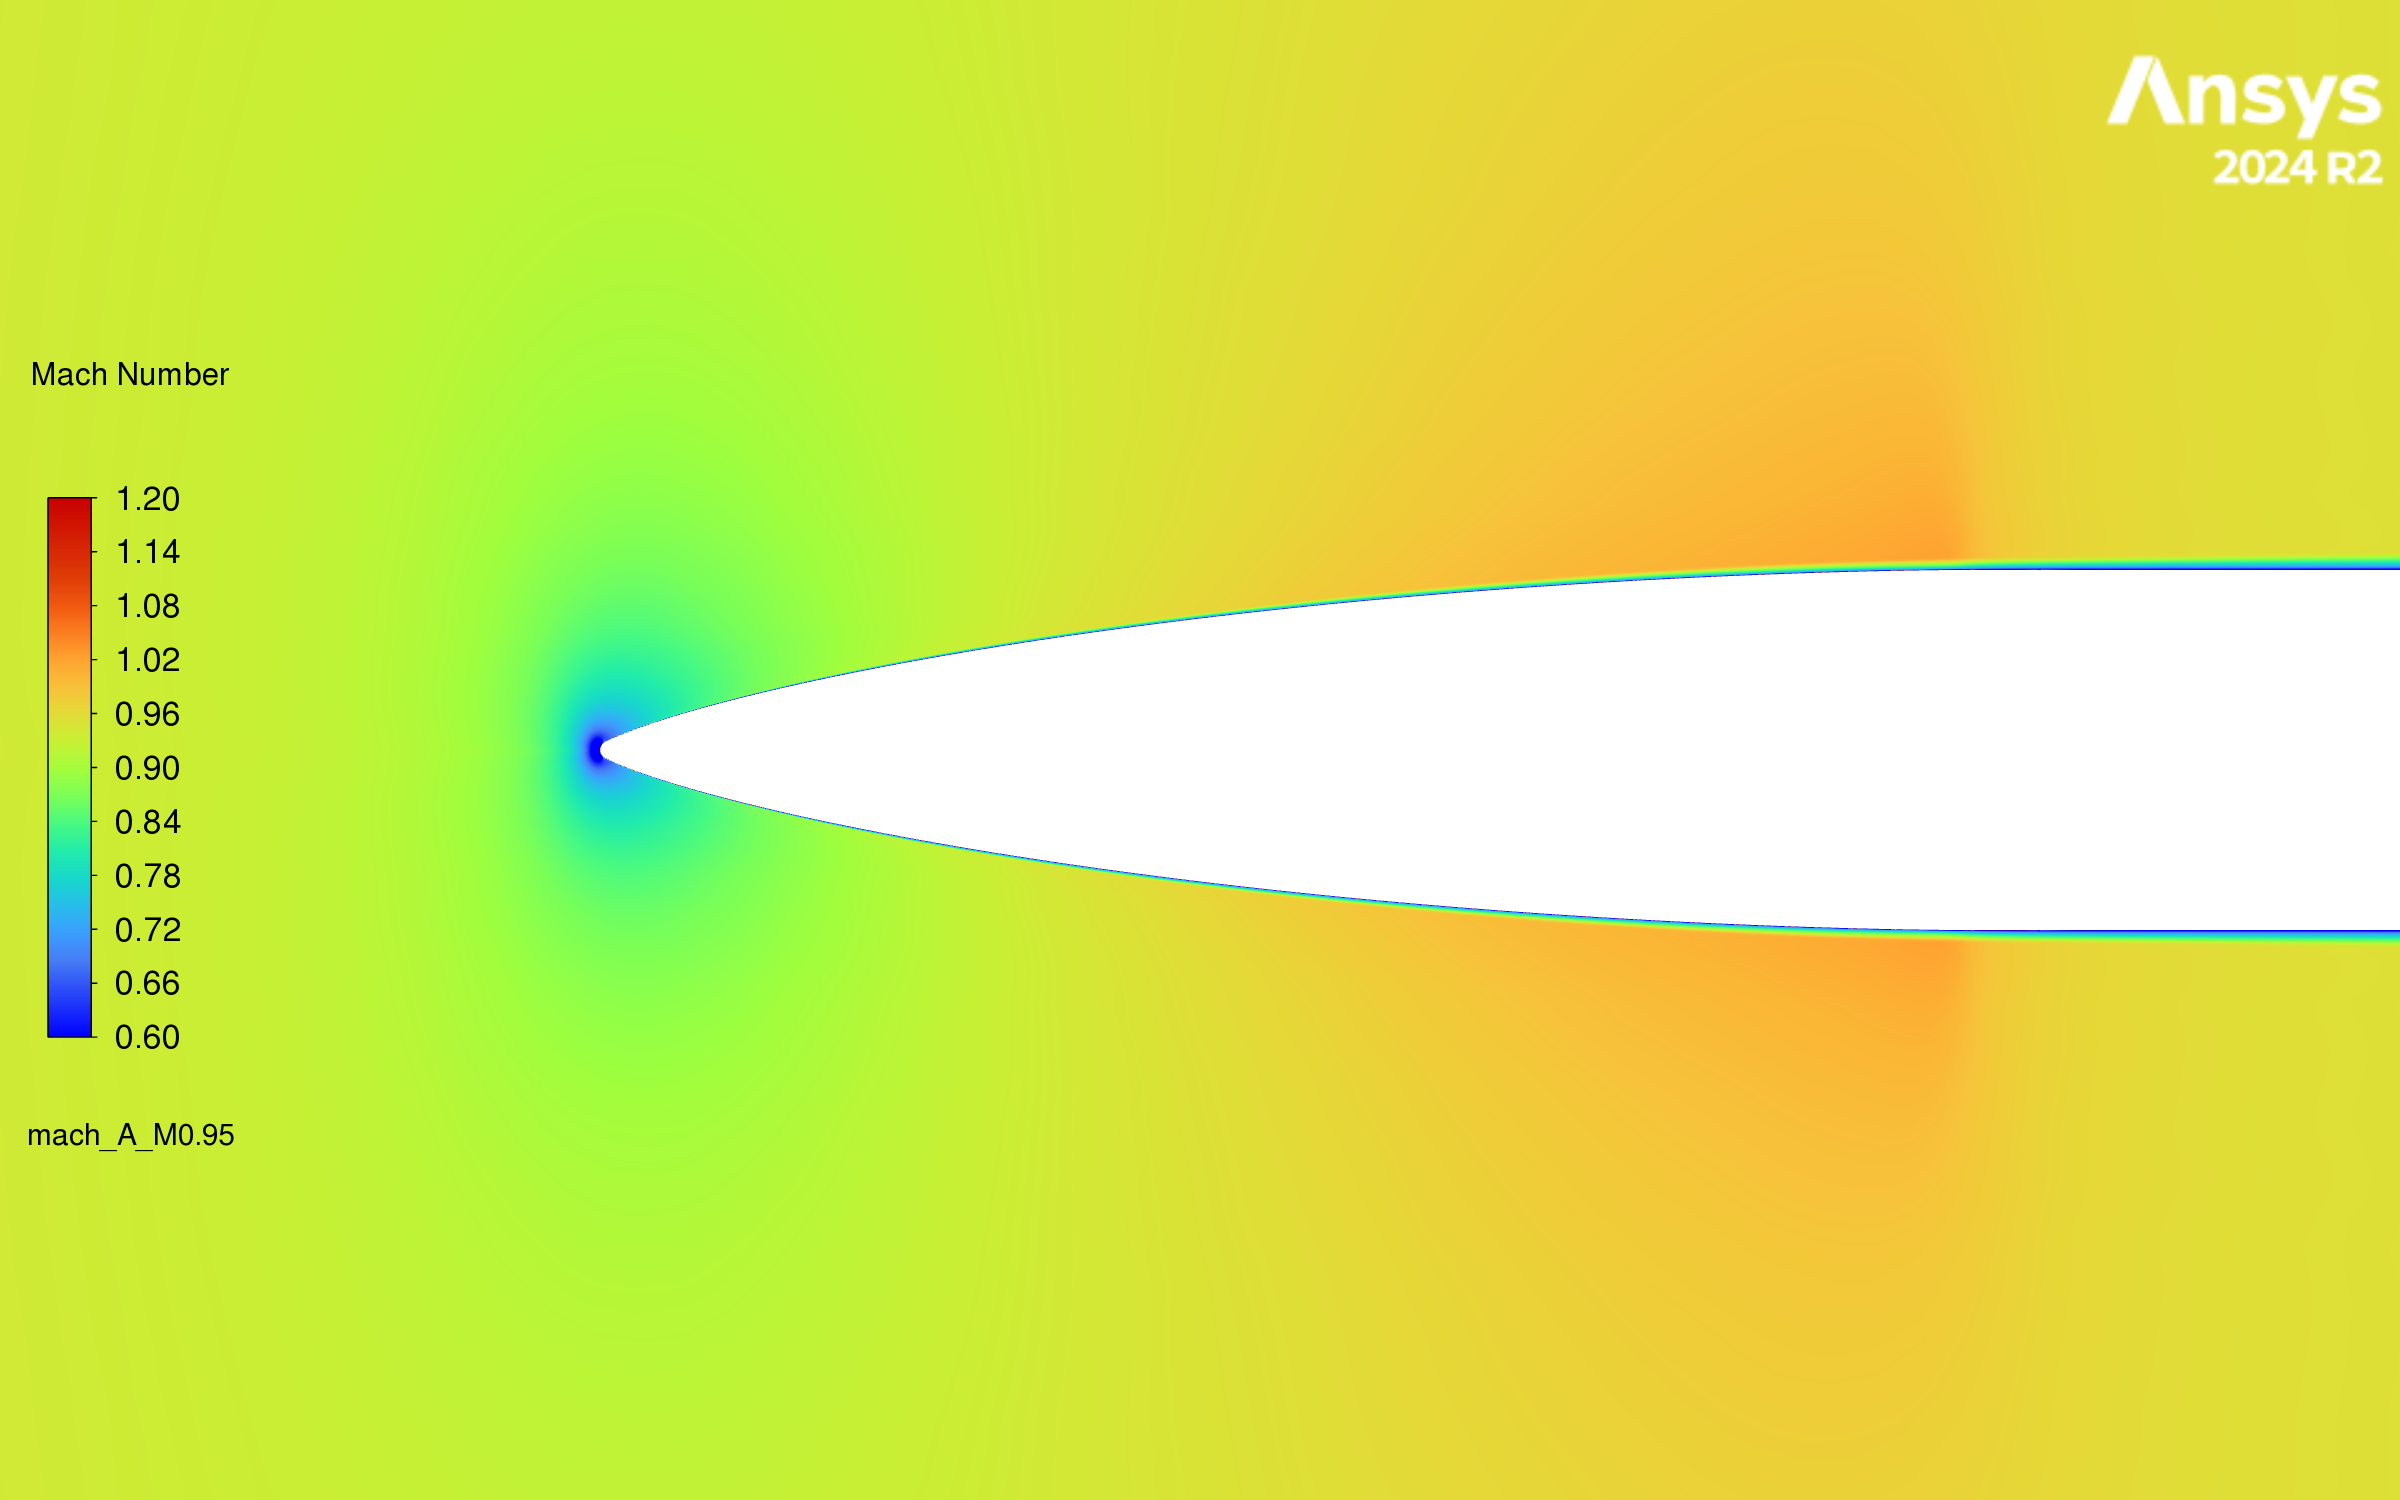
\includegraphics[width=\linewidth]{fluent_mach_A_M0.95}
\caption{Design A.}
\end{subfigure}\hfill
\begin{subfigure}[t]{0.49\linewidth}
\centering
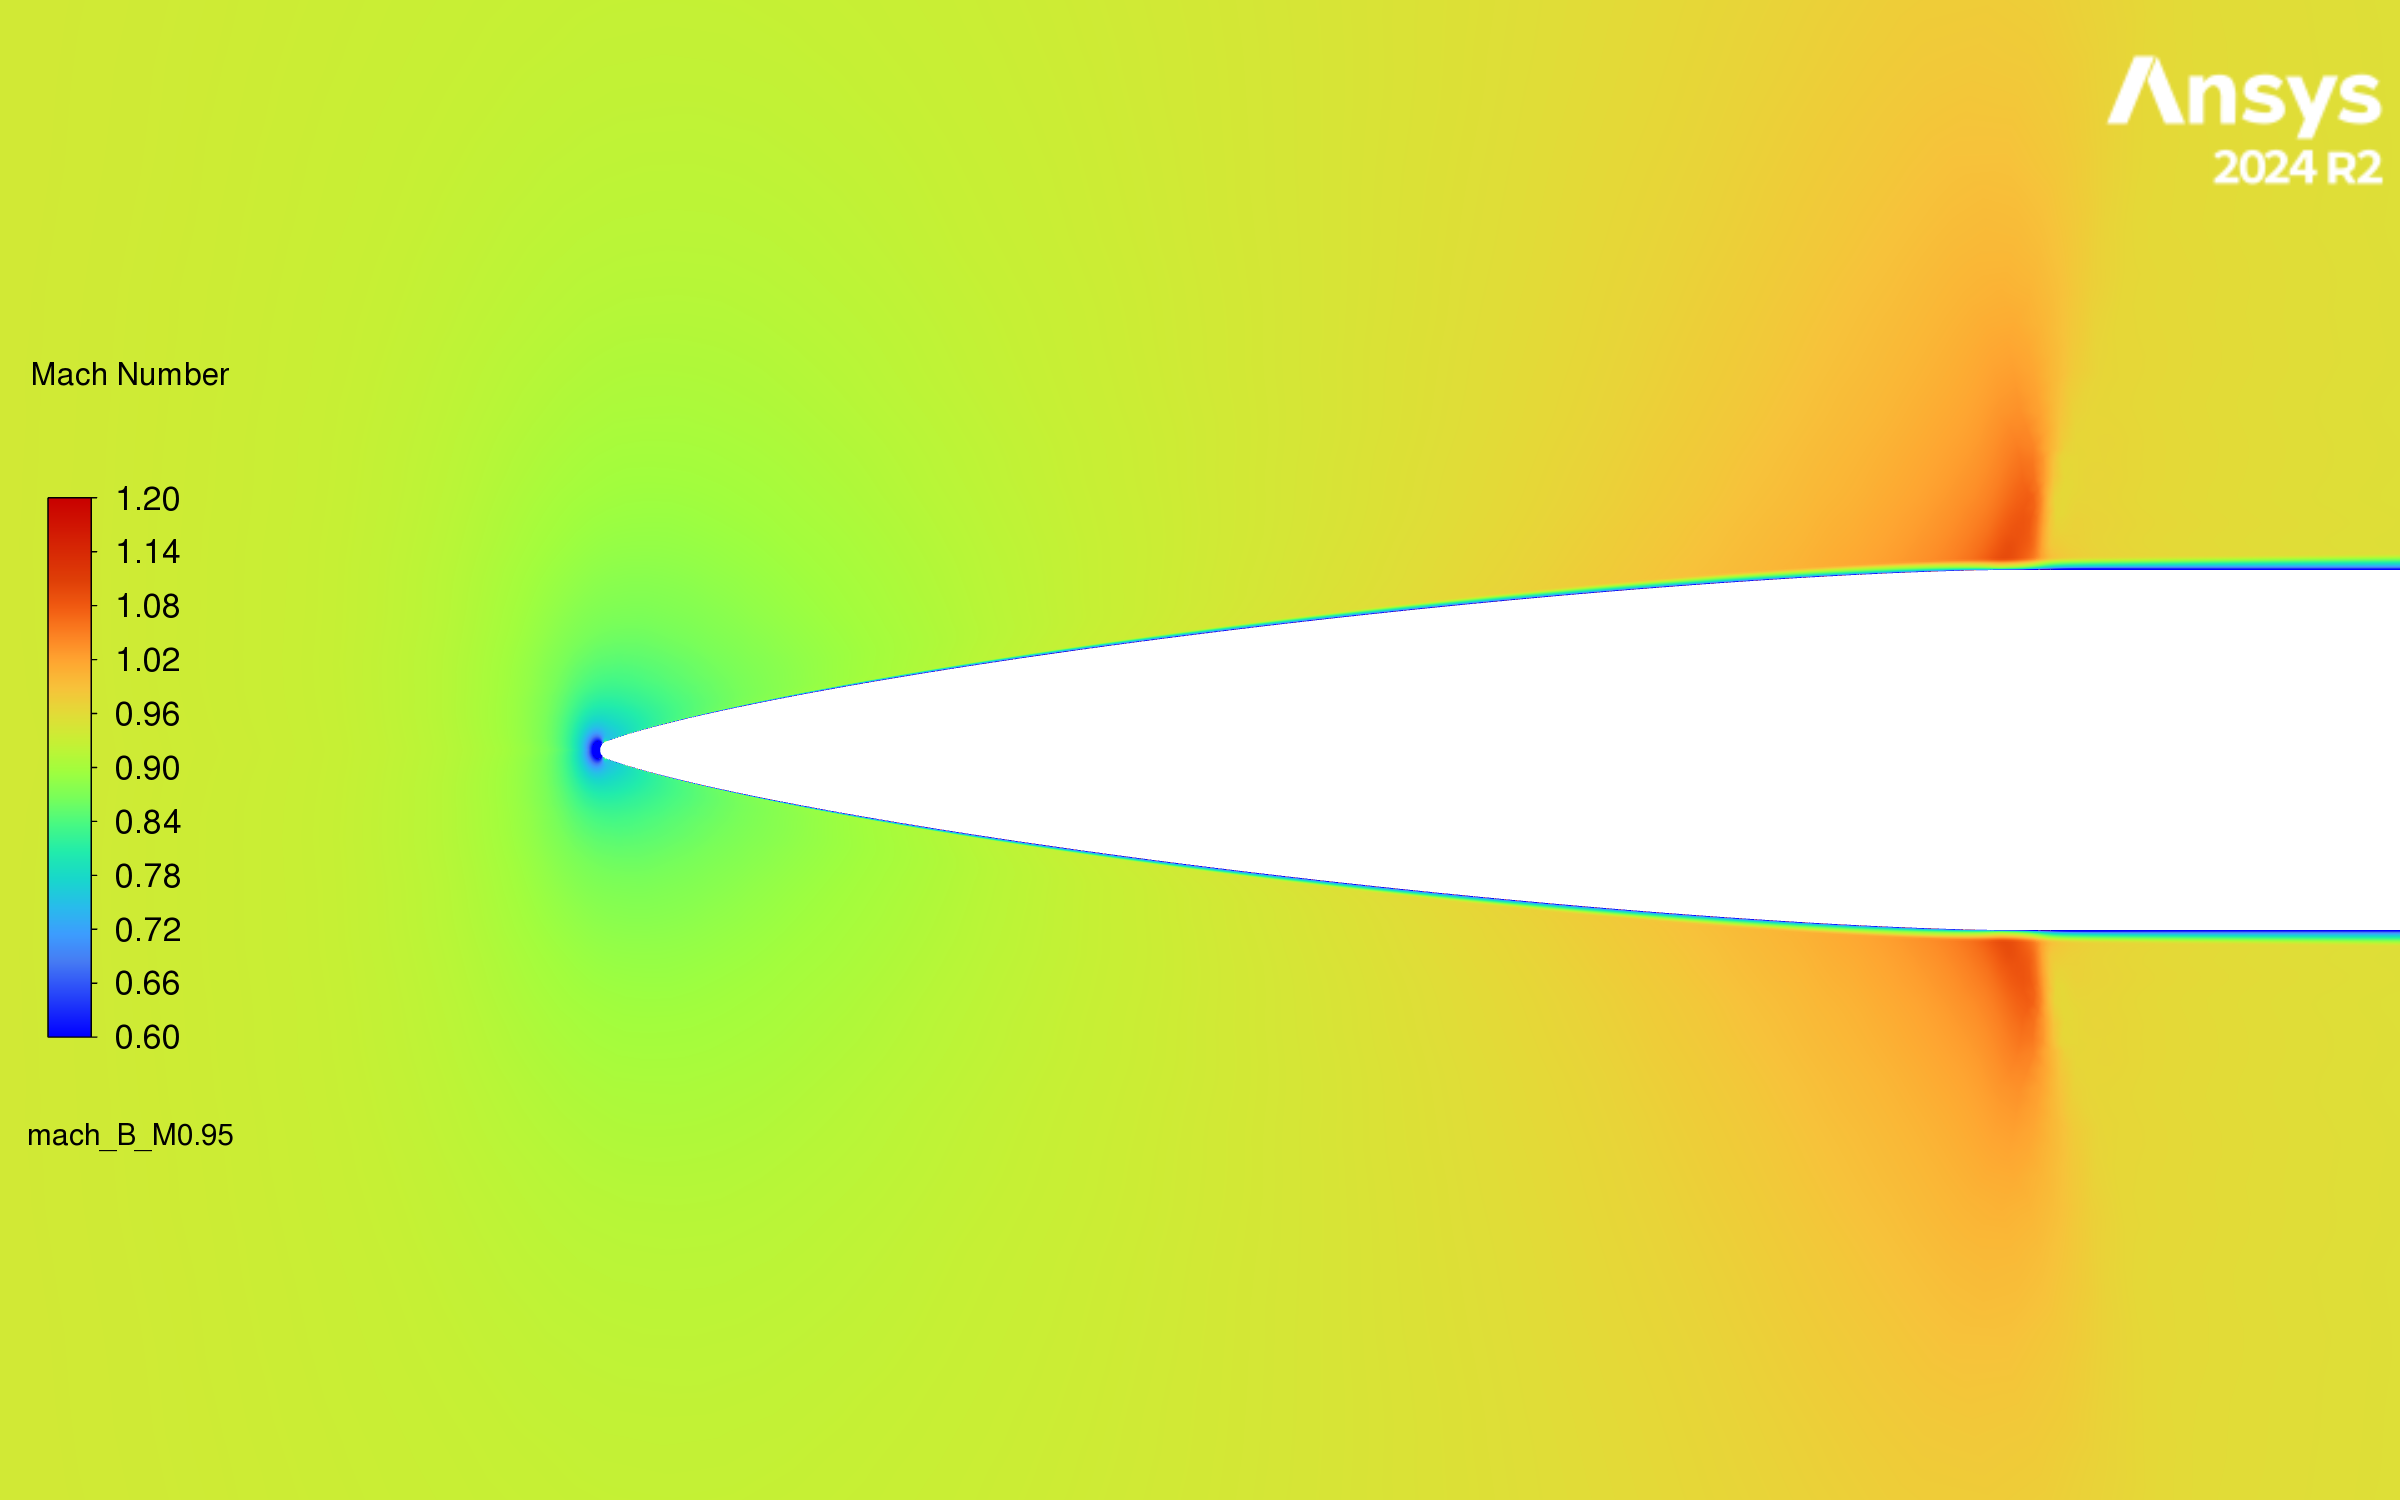
\includegraphics[width=\linewidth]{fluent_mach_B_M0.95}
\caption{Design B.}
\end{subfigure}
\caption{Mach number around the nose at $M = 0.95$ (Fluent). The air speeds up over the shoulder.}
\label{fig:mach095}
\end{figure}

\begin{figure}[H]
\centering
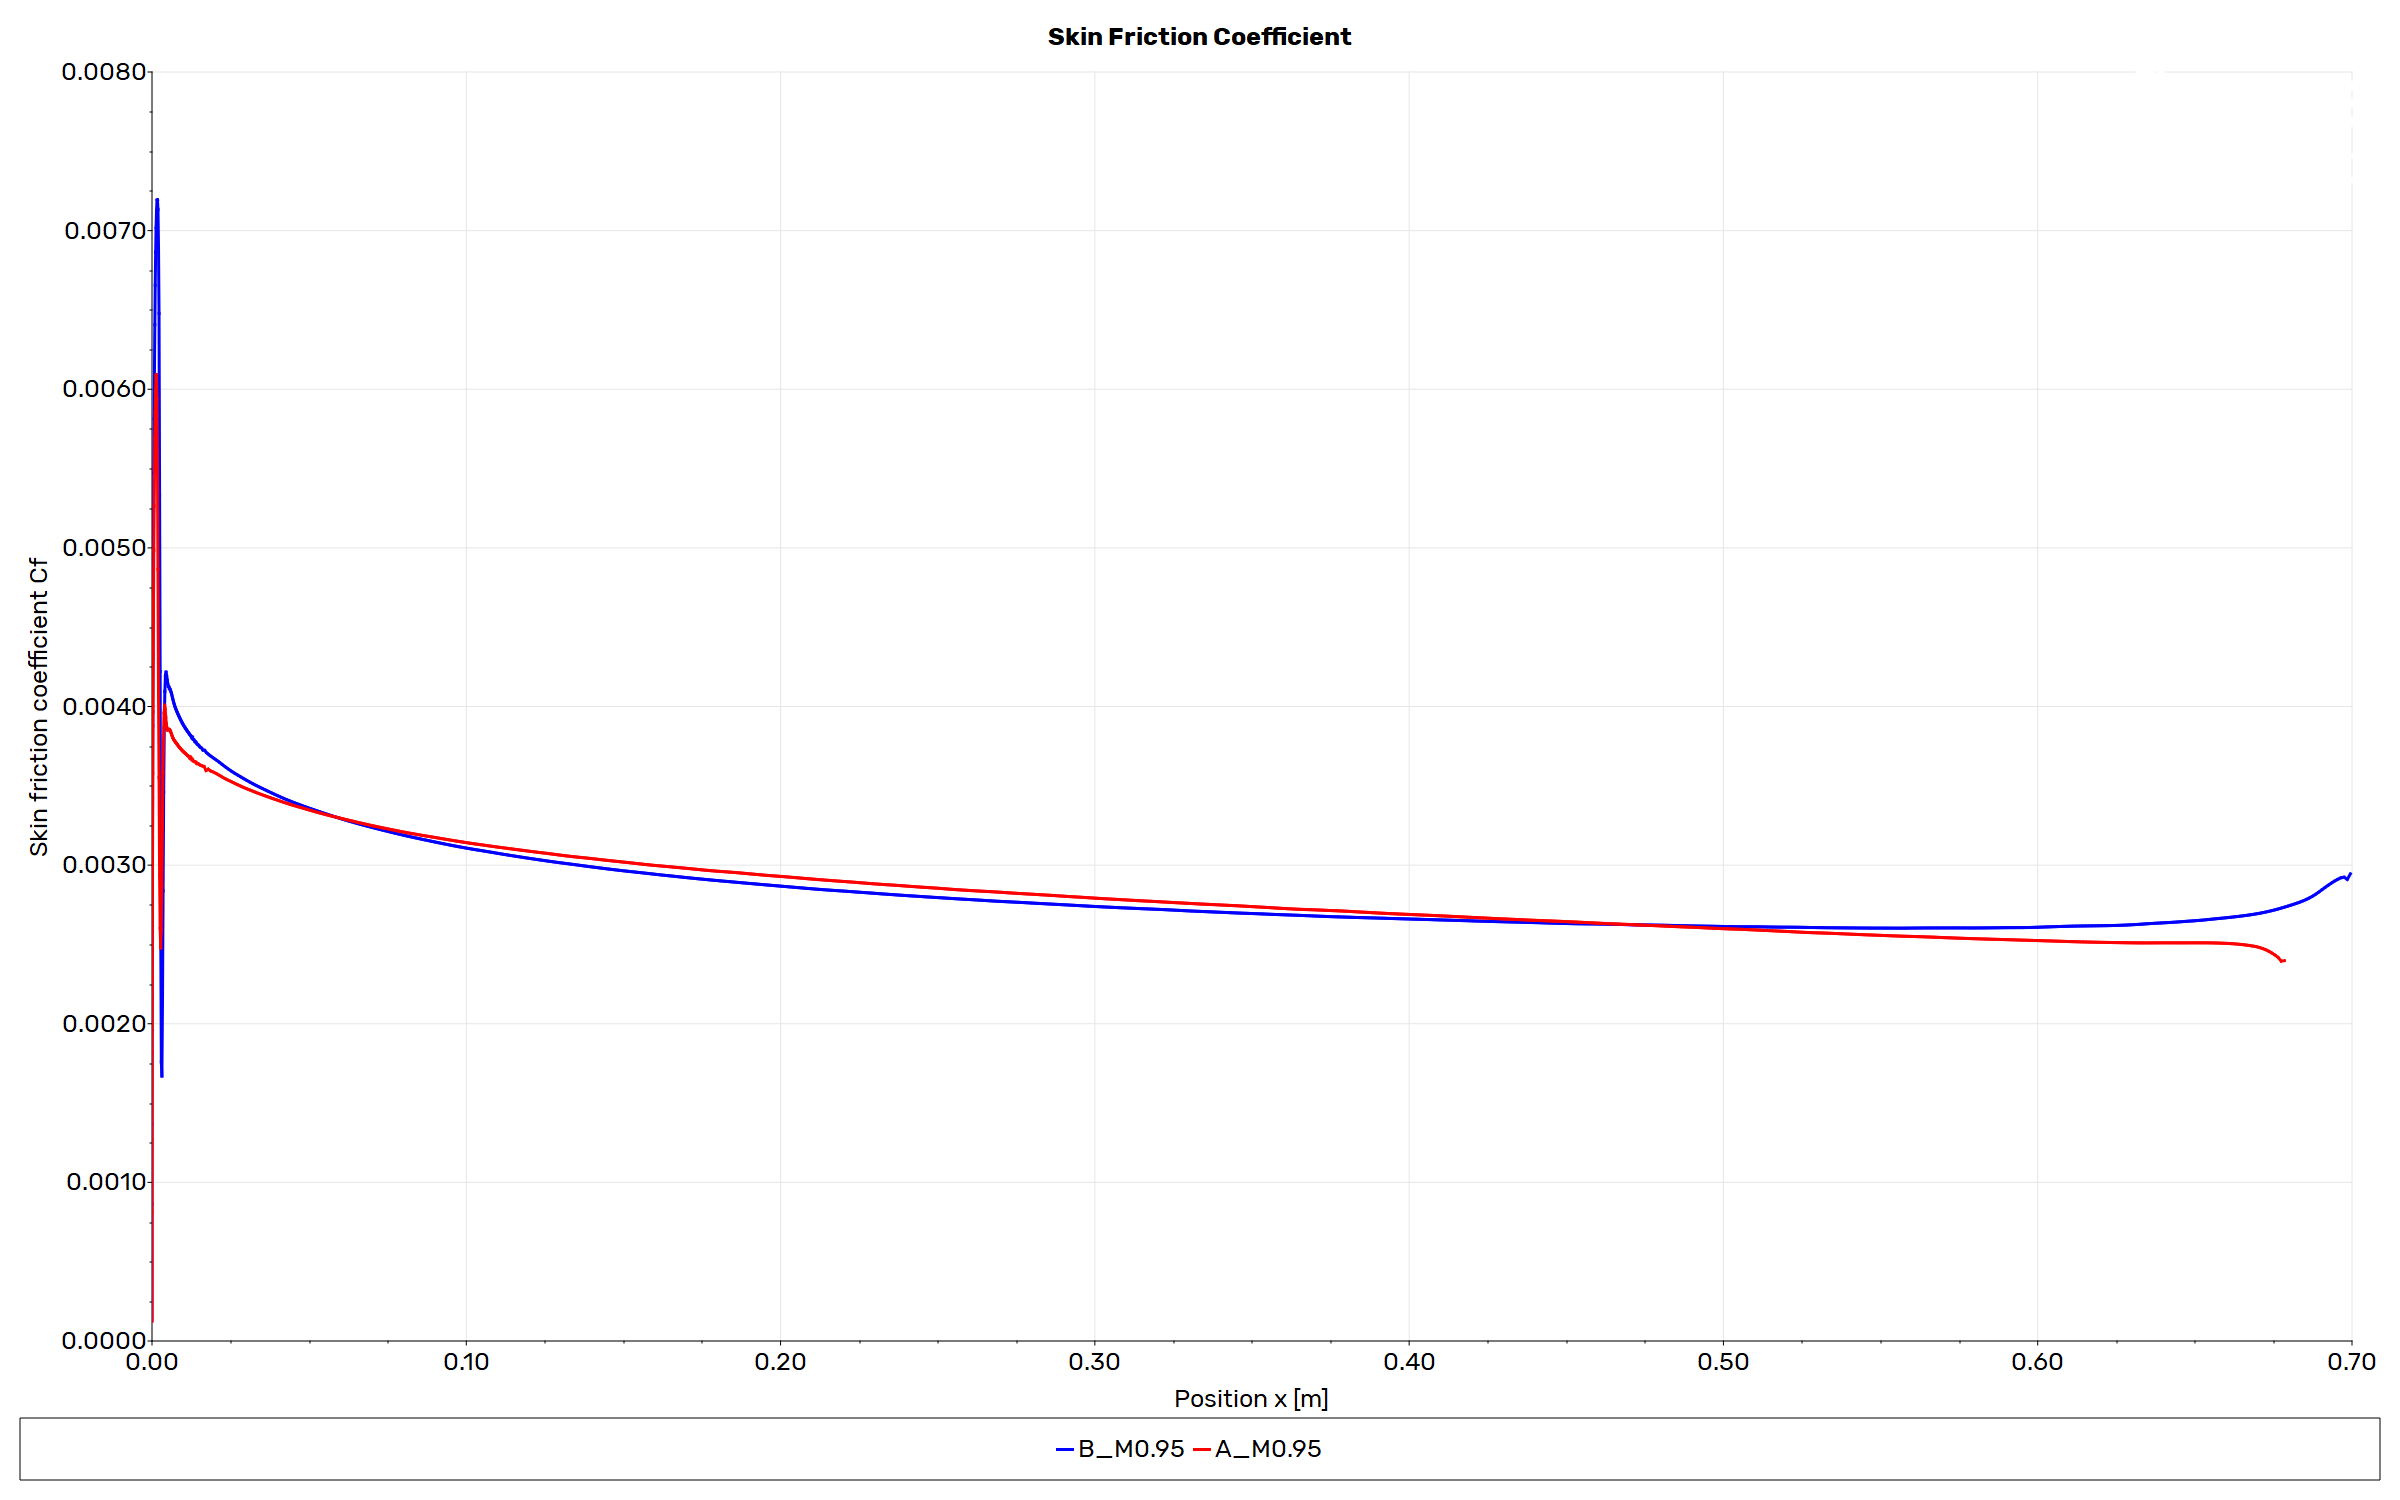
\includegraphics[width=\linewidth]{fluent_cf_AB_M0.95}
\caption{Skin-friction coefficient along the wall at \(M = 0.95\), design A (red) and B (blue), Fluent.}
\label{fig:cf}
\end{figure}

\subsection{Drag over the whole flight}

The flight model uses a drag curve against Mach number. With the start of the drag rise moved from
$M = 0.8$ to 0.94 (report~2 used 0.8), it matches Fluent at all three points within
\SI{5}{\percent} (Figure~\ref{fig:cd}; details in Appendix~\ref{app:dragmethod}). The drag force then
follows the dynamic pressure and peaks at burnout (Figure~\ref{fig:axial}). With the \SI{20}{\micro m}
roughness of the flight model the burnout drag is within \SI{2}{\percent} of Fluent's smooth wall.

\begin{figure}[H]
\centering
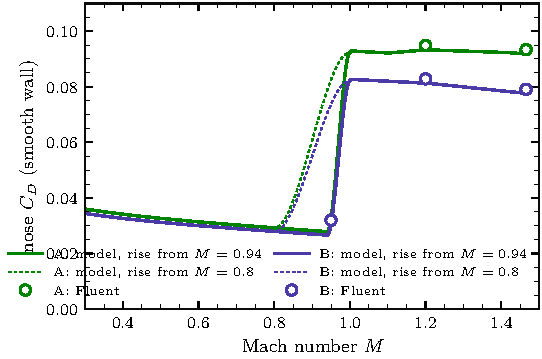
\includegraphics[width=0.75\linewidth]{fig_cd_mach}
\caption{Drag coefficient of the nose against Mach number: flight model with the old (dotted) and new
(solid) start of the drag rise, and Fluent (circles). Design A in green, B in purple; smooth wall in both.}
\label{fig:cd}
\end{figure}

\begin{figure}[H]
\centering
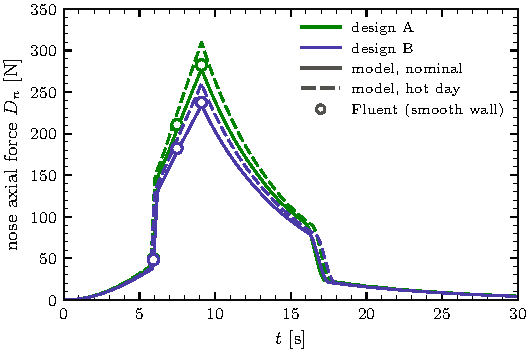
\includegraphics[width=0.75\linewidth]{fig_axial_force}
\caption{Drag of the nose during the flight (flight model, rough wall) and the Fluent points (smooth
wall).}
\label{fig:axial}
\end{figure}
